\chapter{Annexes}

\section{Inventaire des pièces justificatives}
Les annexes sont destinées à fournir des preuves utiles, sans reproduire l'intégralité de la correspondance ni divulguer inutilement des coordonnées personnelles. Les noms des interlocuteurs institutionnels sont conservés dans le corps du mémoire lorsqu'ils sont nécessaires à la compréhension de la démarche ; les adresses privées, numéros de téléphone et identifiants sont à masquer sur toute copie diffusée.

\begin{longtable}{@{}p{0.13\textwidth}p{0.57\textwidth}p{0.20\textwidth}@{}}
\toprule
\rowcolor{bleuECSR}
\textcolor{white}{\textbf{Repère}} & \textcolor{white}{\textbf{Pièce à classer}} & \textcolor{white}{\textbf{Situation}} \\
\midrule
\endfirsthead
\toprule
\rowcolor{bleuECSR}
\textcolor{white}{\textbf{Repère}} & \textcolor{white}{\textbf{Pièce à classer}} & \textcolor{white}{\textbf{Situation}} \\ \midrule
\endhead
A1 & Courriel de proposition du 9 septembre 2026 et réponse favorable du 10 septembre. & Disponible \\
A2 & Questionnaire de recueil des besoins commanditaire et réponse transmise le 29 septembre. & Disponible \\
A3 & Courriels des 28--29 septembre : demande d'entretien, correction de date et confirmation du rendez-vous du 1\textsuperscript{er} octobre. & Disponible \\
A4 & Questionnaire anonyme de 30 questions adressé aux stagiaires le 26 octobre. & Disponible \\
A5 & Courriels du 26 et du 29 octobre relatifs à la diffusion, la relance et la transmission annoncée des réponses. & Disponible \\
A6 & Synthèse agrégée des treize réponses et graphique comparatif des besoins. & Disponible \\
A7 & Demande de matériel du 11 octobre et réponse du Bureau de la sécurité routière du 12 octobre. & Disponible \\
A8 & Convention de prêt envoyée le 30 octobre ; convention contresignée et transmise le 10 novembre ; échanges des 10--12 novembre sur les dates et horaires de retrait et restitution et demande d'accès au CADAM. & Échanges disponibles ; exécution à confirmer \\
A9 & Diaporama initial « Sur la route du chantier --- Alcool et distracteurs » et support de 30 pages « Smartphone au volant : le piège des chantiers » (version du 13 novembre 2026). & Disponibles \\
A10 & Tableau synoptique prévisionnel de deux heures ; protocole extérieur « Même parcours, attention différente » et grille vierge d’observation. & Rédigés ; à valider \\
A11 & Grille d'évaluation des acquis et questionnaire de satisfaction utilisés. & À finaliser \\
A12 & Bilan de l'action, retour commanditaire et autoanalyse. & Après le 4 déc. \\
\bottomrule
\end{longtable}



\section{Échanges avec le commanditaire : premier contact (A1)}
Courriels qui documentent la proposition initiale et la transmission du premier questionnaire.

\clearpage
\begin{landscape}
\thispagestyle{plain}
\noindent{\large\bfseries 9 septembre 2026 — Proposition initiale de sensibilisation}\par\medskip
\begin{center}
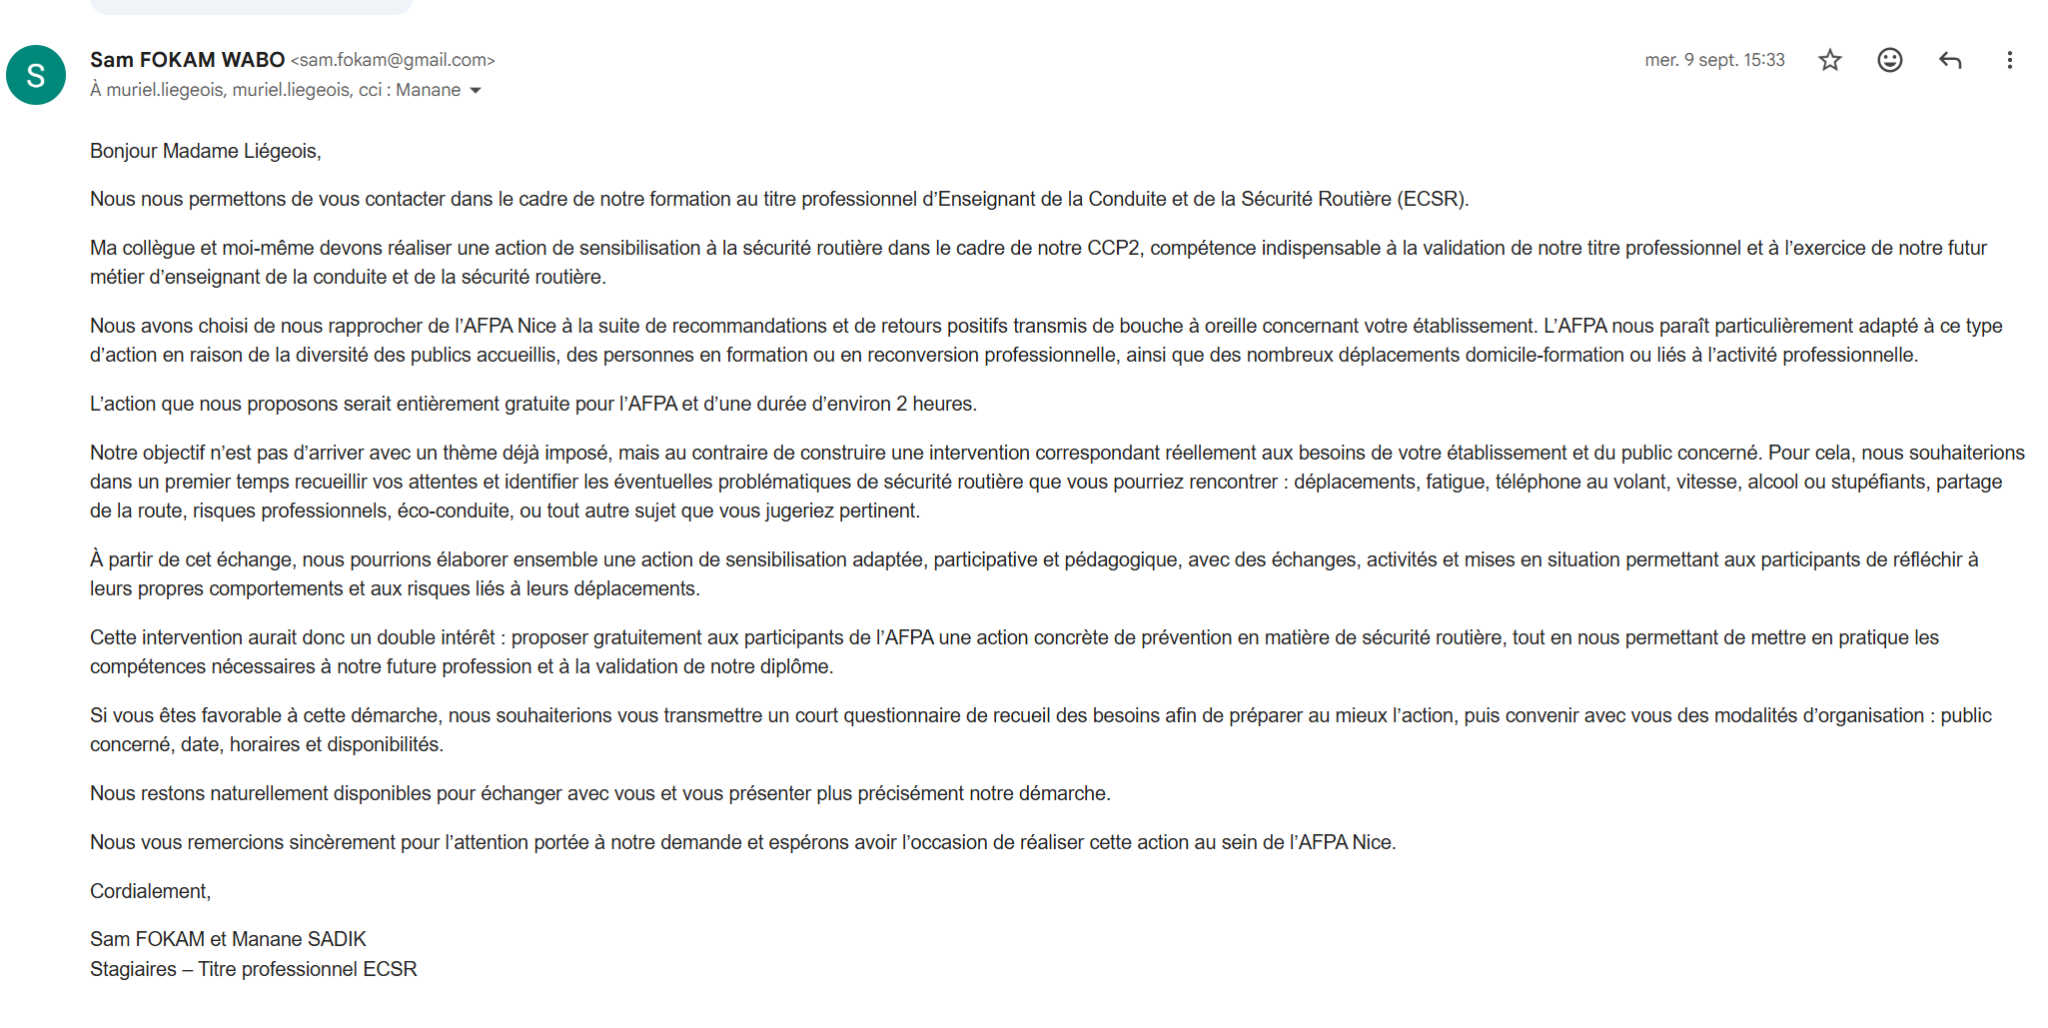
\includegraphics[width=0.97\linewidth,height=0.77\textheight,keepaspectratio]{images/annexes/echanges/a01_20260909_proposition.png}
\end{center}
\end{landscape}

\clearpage
\begin{landscape}
\thispagestyle{plain}
\noindent{\large\bfseries 10 septembre — Réponse favorable de Mme Liégeois}\par\medskip
\begin{center}
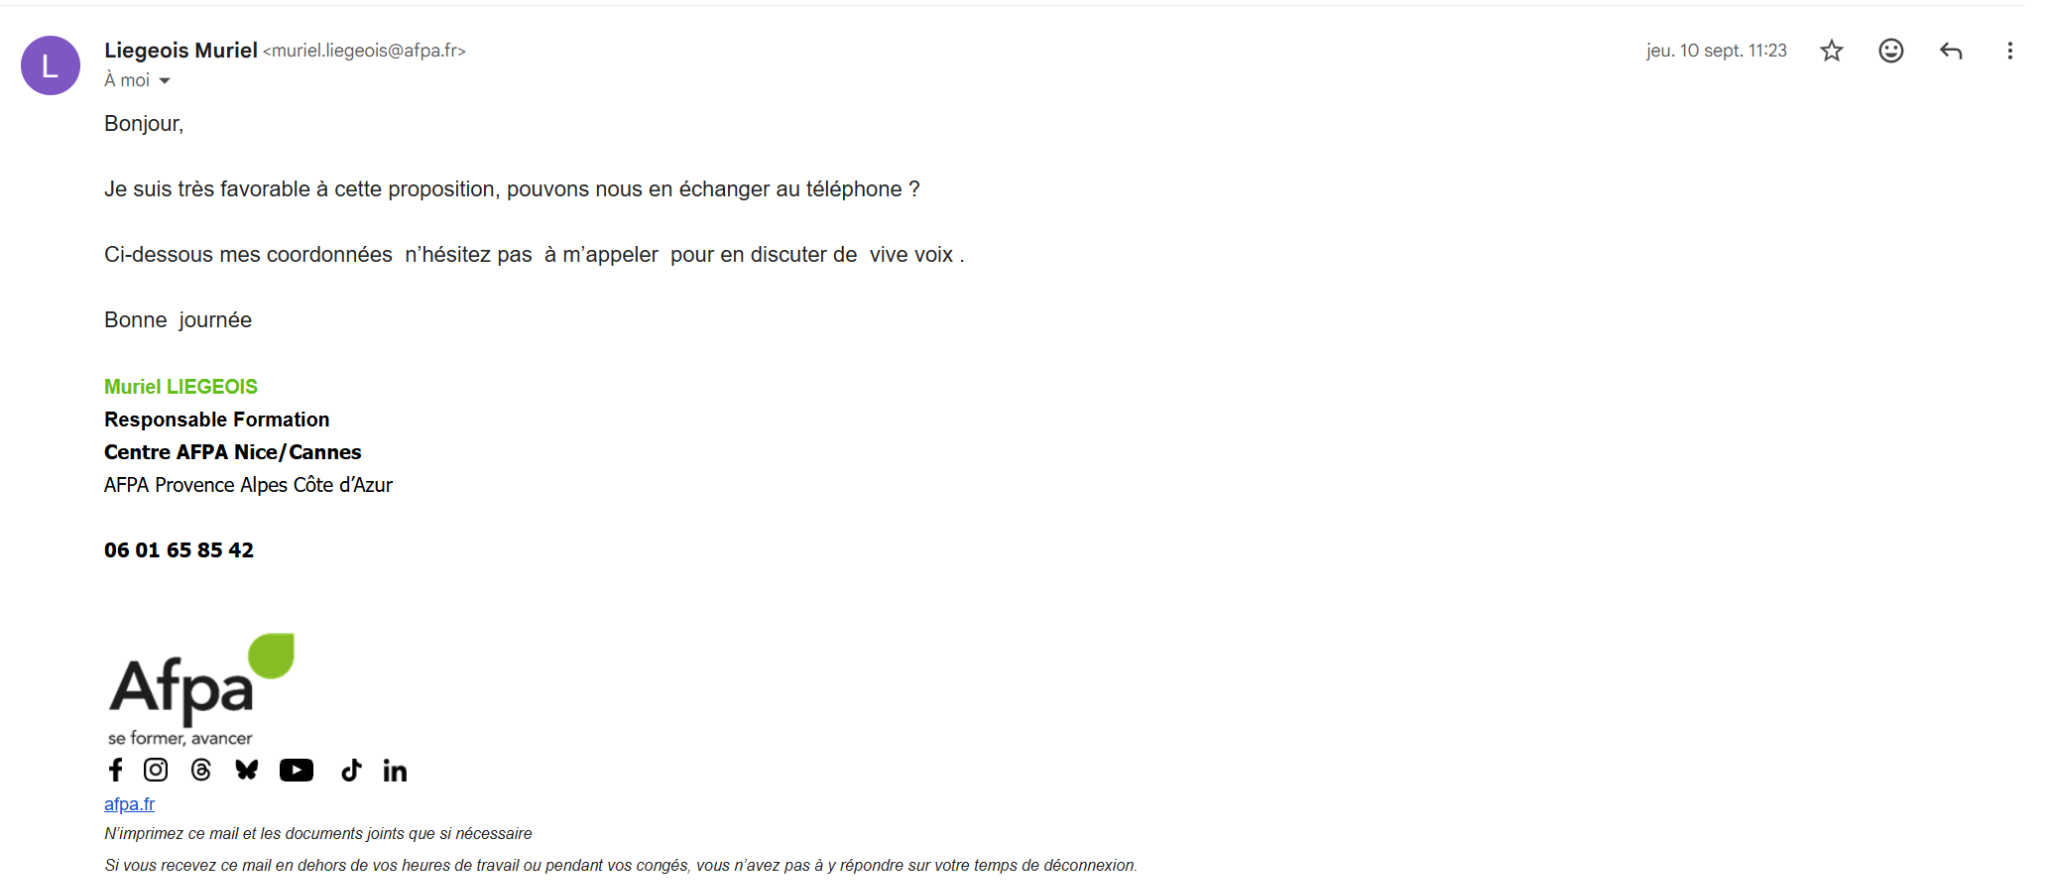
\includegraphics[width=0.97\linewidth,height=0.77\textheight,keepaspectratio]{images/annexes/echanges/a02_20260910_accord.png}
\end{center}
\end{landscape}

\clearpage
\begin{landscape}
\thispagestyle{plain}
\noindent{\large\bfseries 11 septembre — Premier envoi annoncé du questionnaire}\par\medskip
\begin{center}
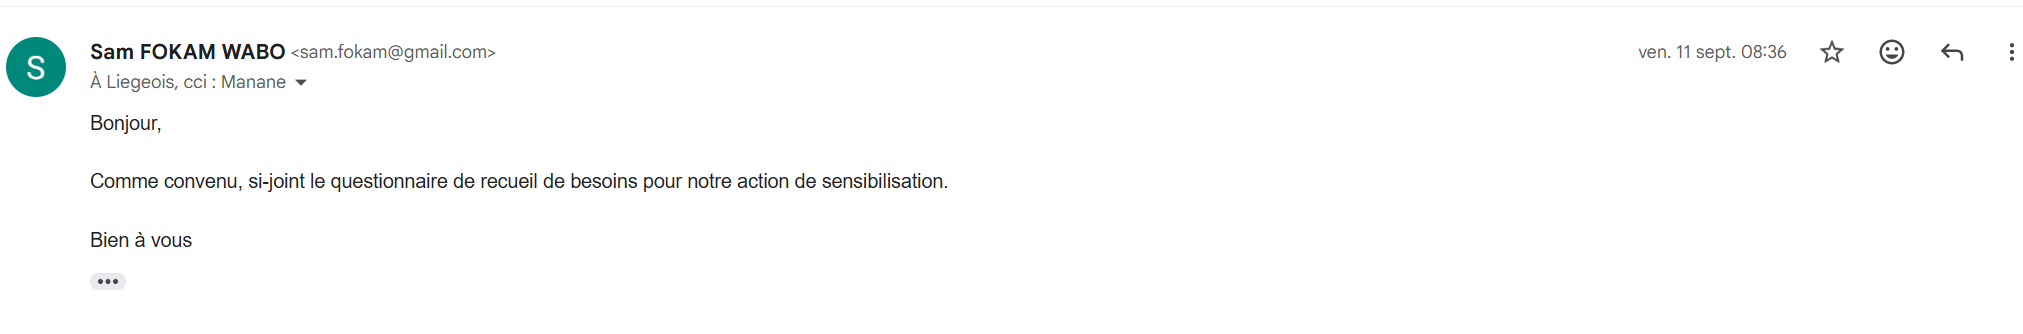
\includegraphics[width=0.97\linewidth,height=0.77\textheight,keepaspectratio]{images/annexes/echanges/a03_20260911_envoi_quest.png}
\end{center}
\end{landscape}

\clearpage
\begin{landscape}
\thispagestyle{plain}
\noindent{\large\bfseries 11 septembre — Signalement de la pièce jointe manquante}\par\medskip
\begin{center}
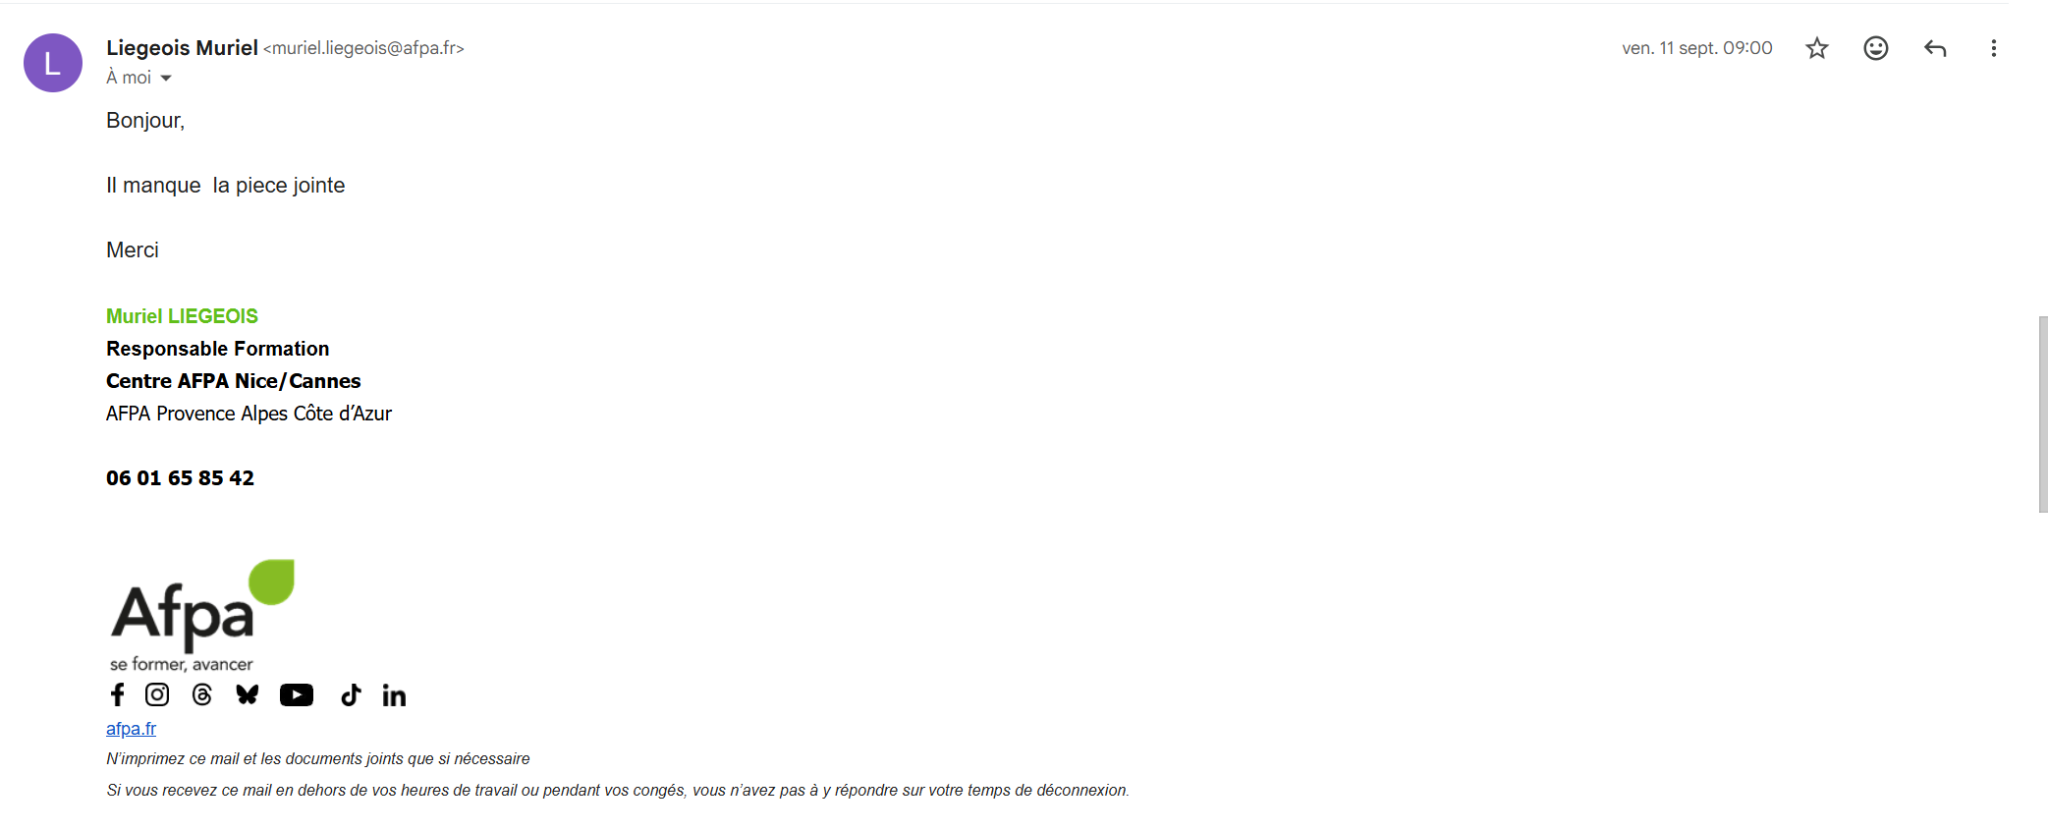
\includegraphics[width=0.97\linewidth,height=0.77\textheight,keepaspectratio]{images/annexes/echanges/a04_20260911_pj_absente.png}
\end{center}
\end{landscape}

\clearpage
\begin{landscape}
\thispagestyle{plain}
\noindent{\large\bfseries 23 septembre — Transmission effective du questionnaire}\par\medskip
\begin{center}
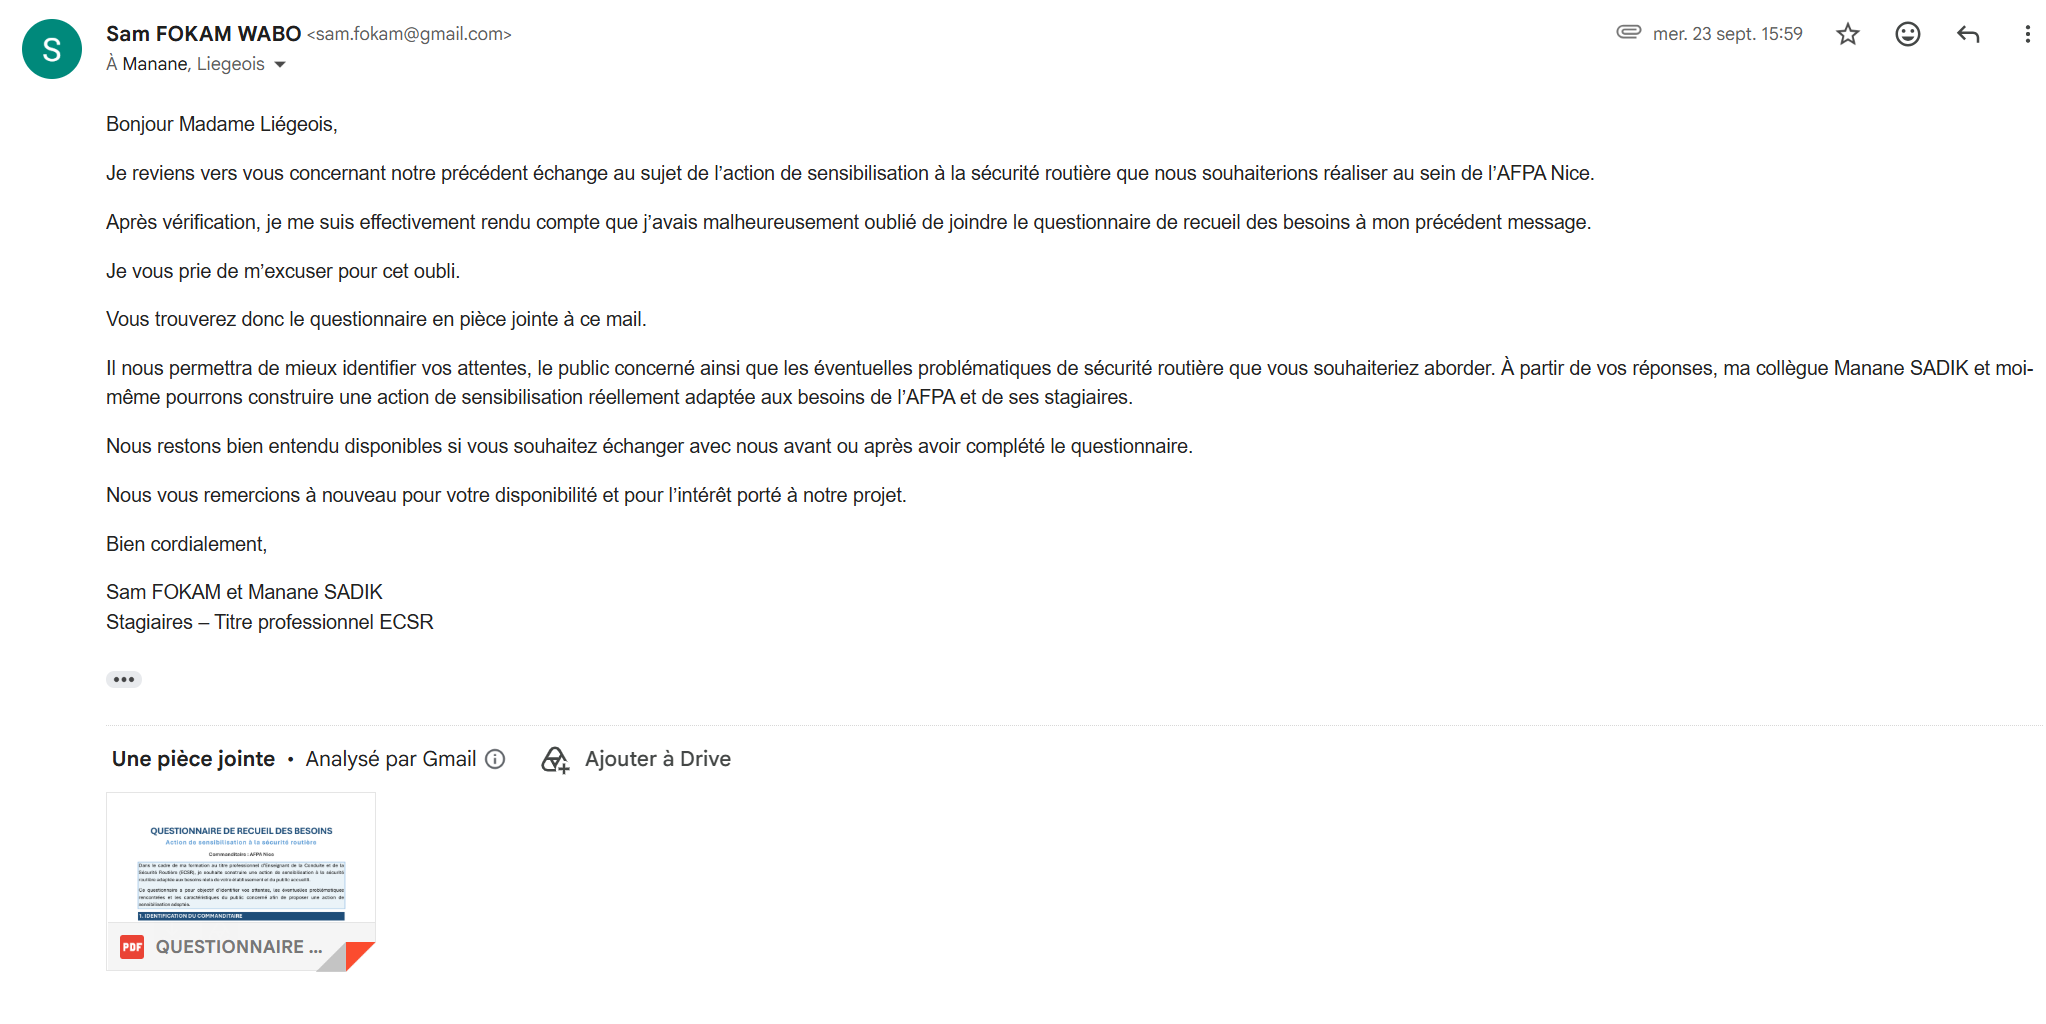
\includegraphics[width=0.97\linewidth,height=0.77\textheight,keepaspectratio]{images/annexes/echanges/a05_20260923_questionnaire.png}
\end{center}
\end{landscape}

\section{Questionnaire de recueil des besoins du commanditaire (A2)}
Les pages suivantes reproduisent, sous forme d'images, le questionnaire de recueil des besoins adressé au commanditaire AFPA. Cette pièce est directement liée à la partie consacrée à l'analyse de la demande et à la clarification du besoin.

\clearpage
\subsection*{Questionnaire commanditaire --- page 1}
\begin{figure}[H]
\centering
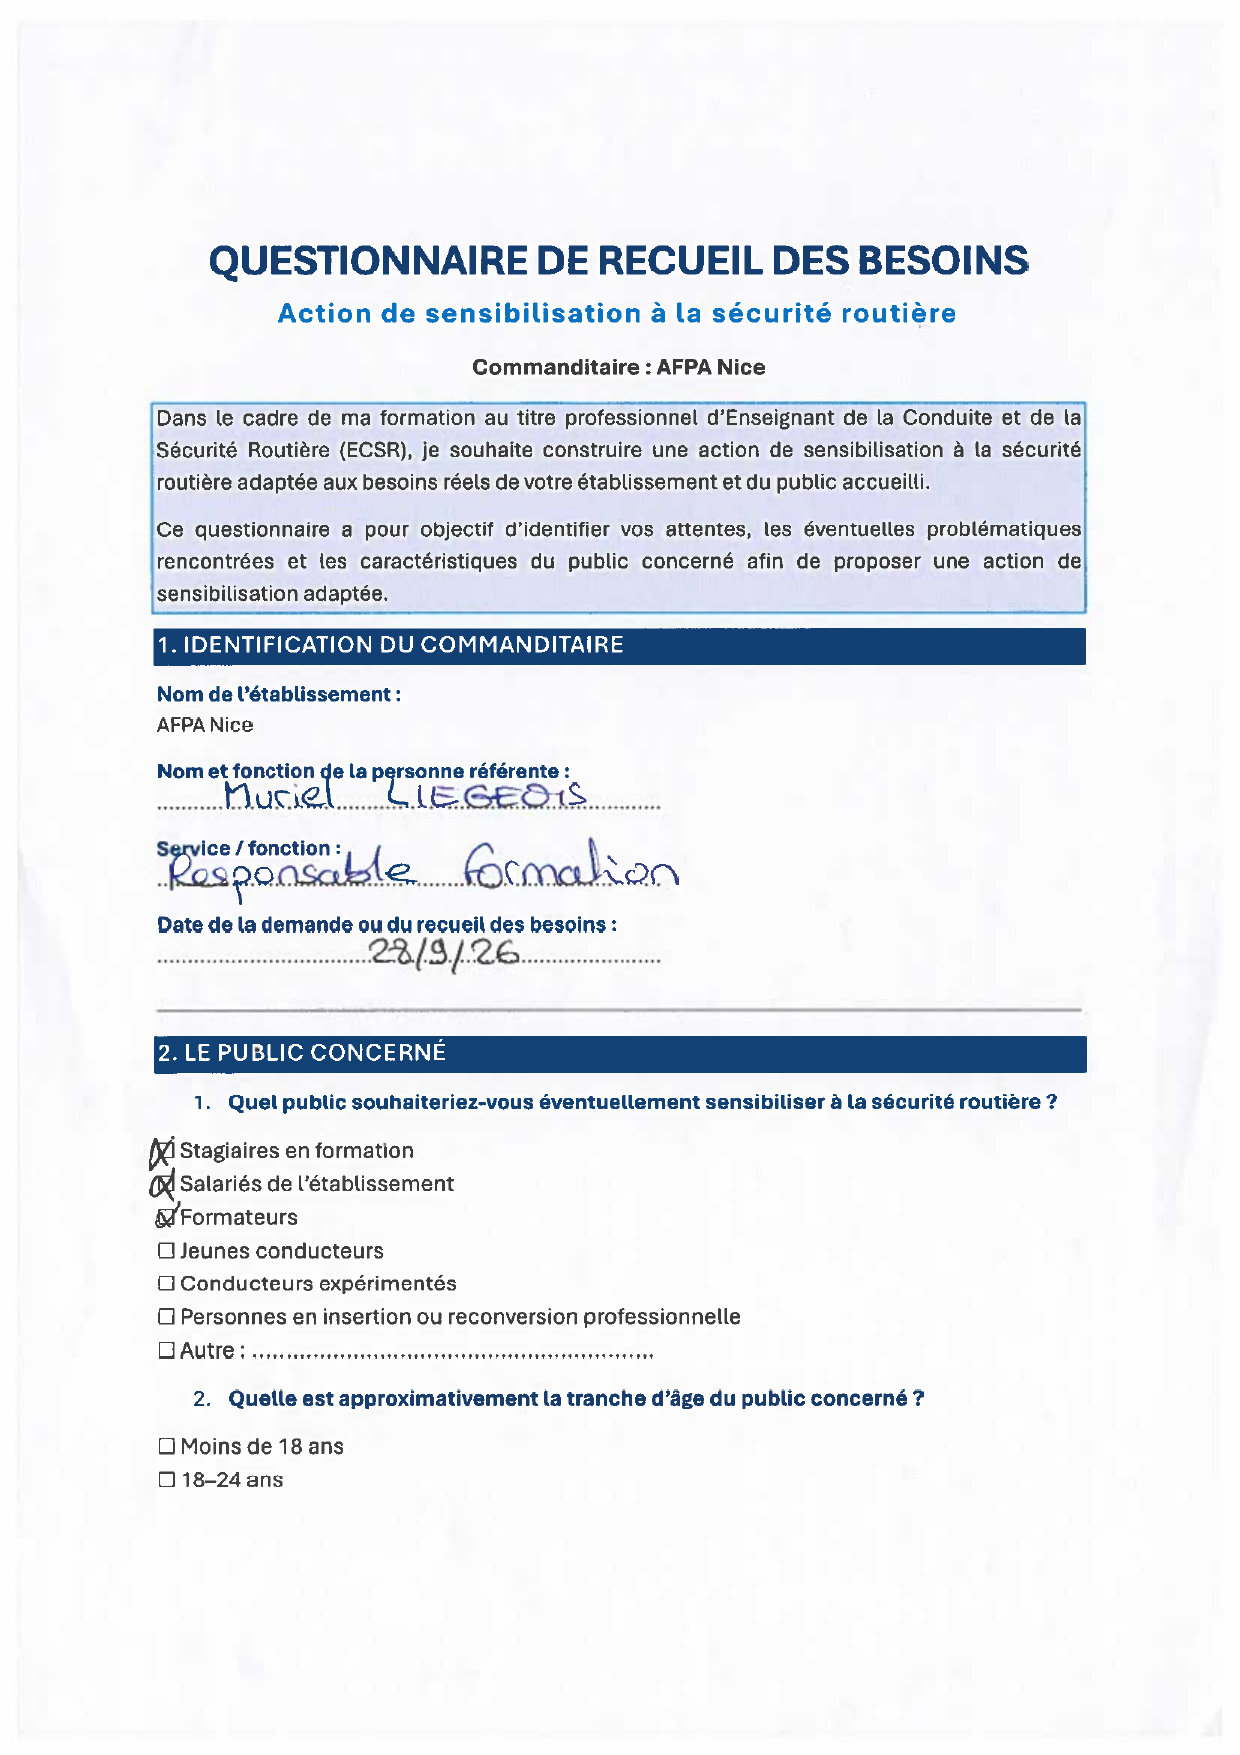
\includegraphics[width=0.92\textwidth]{images/annexes/questionnaire_commanditaire-1.png}
\end{figure}

\clearpage
\subsection*{Questionnaire commanditaire --- page 2}
\begin{figure}[H]
\centering
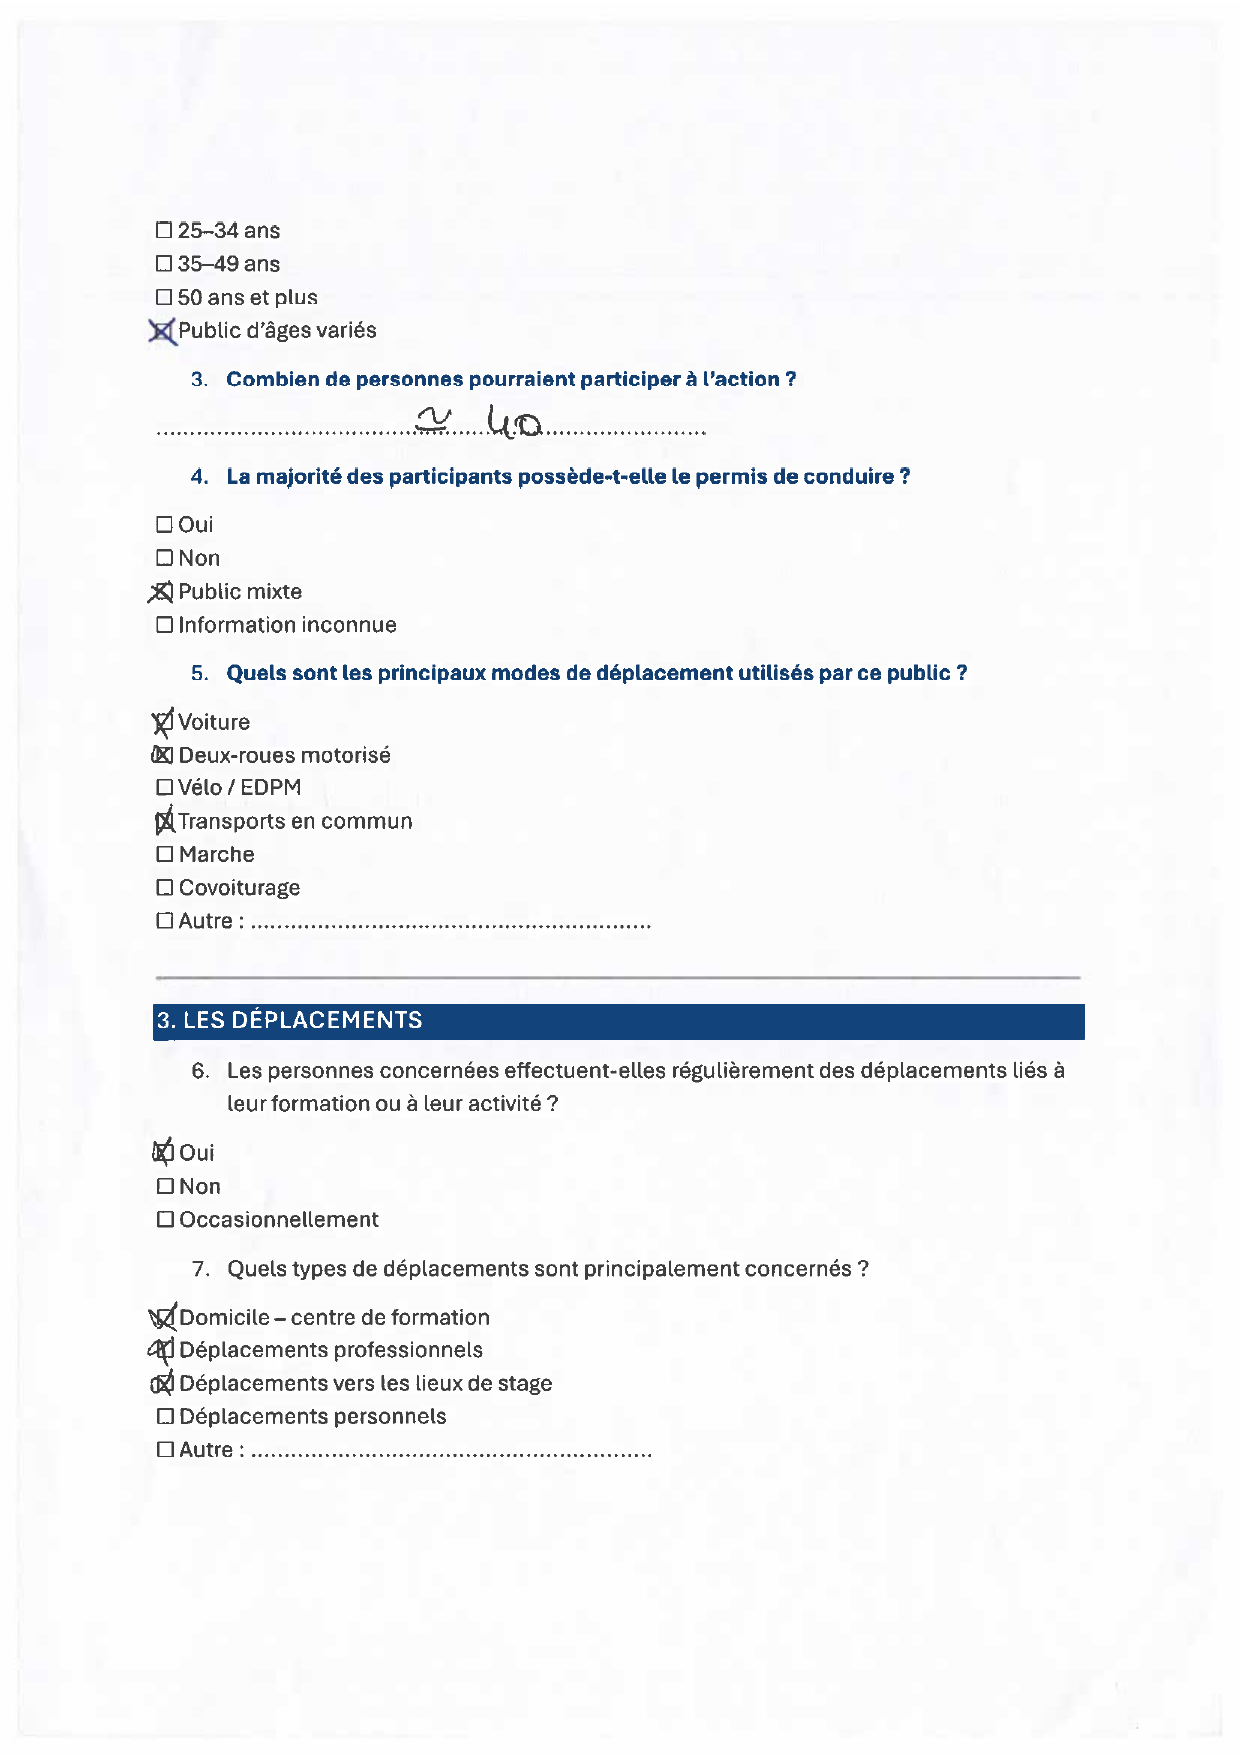
\includegraphics[width=0.92\textwidth]{images/annexes/questionnaire_commanditaire-2.png}
\end{figure}

\clearpage
\subsection*{Questionnaire commanditaire --- page 3}
\begin{figure}[H]
\centering
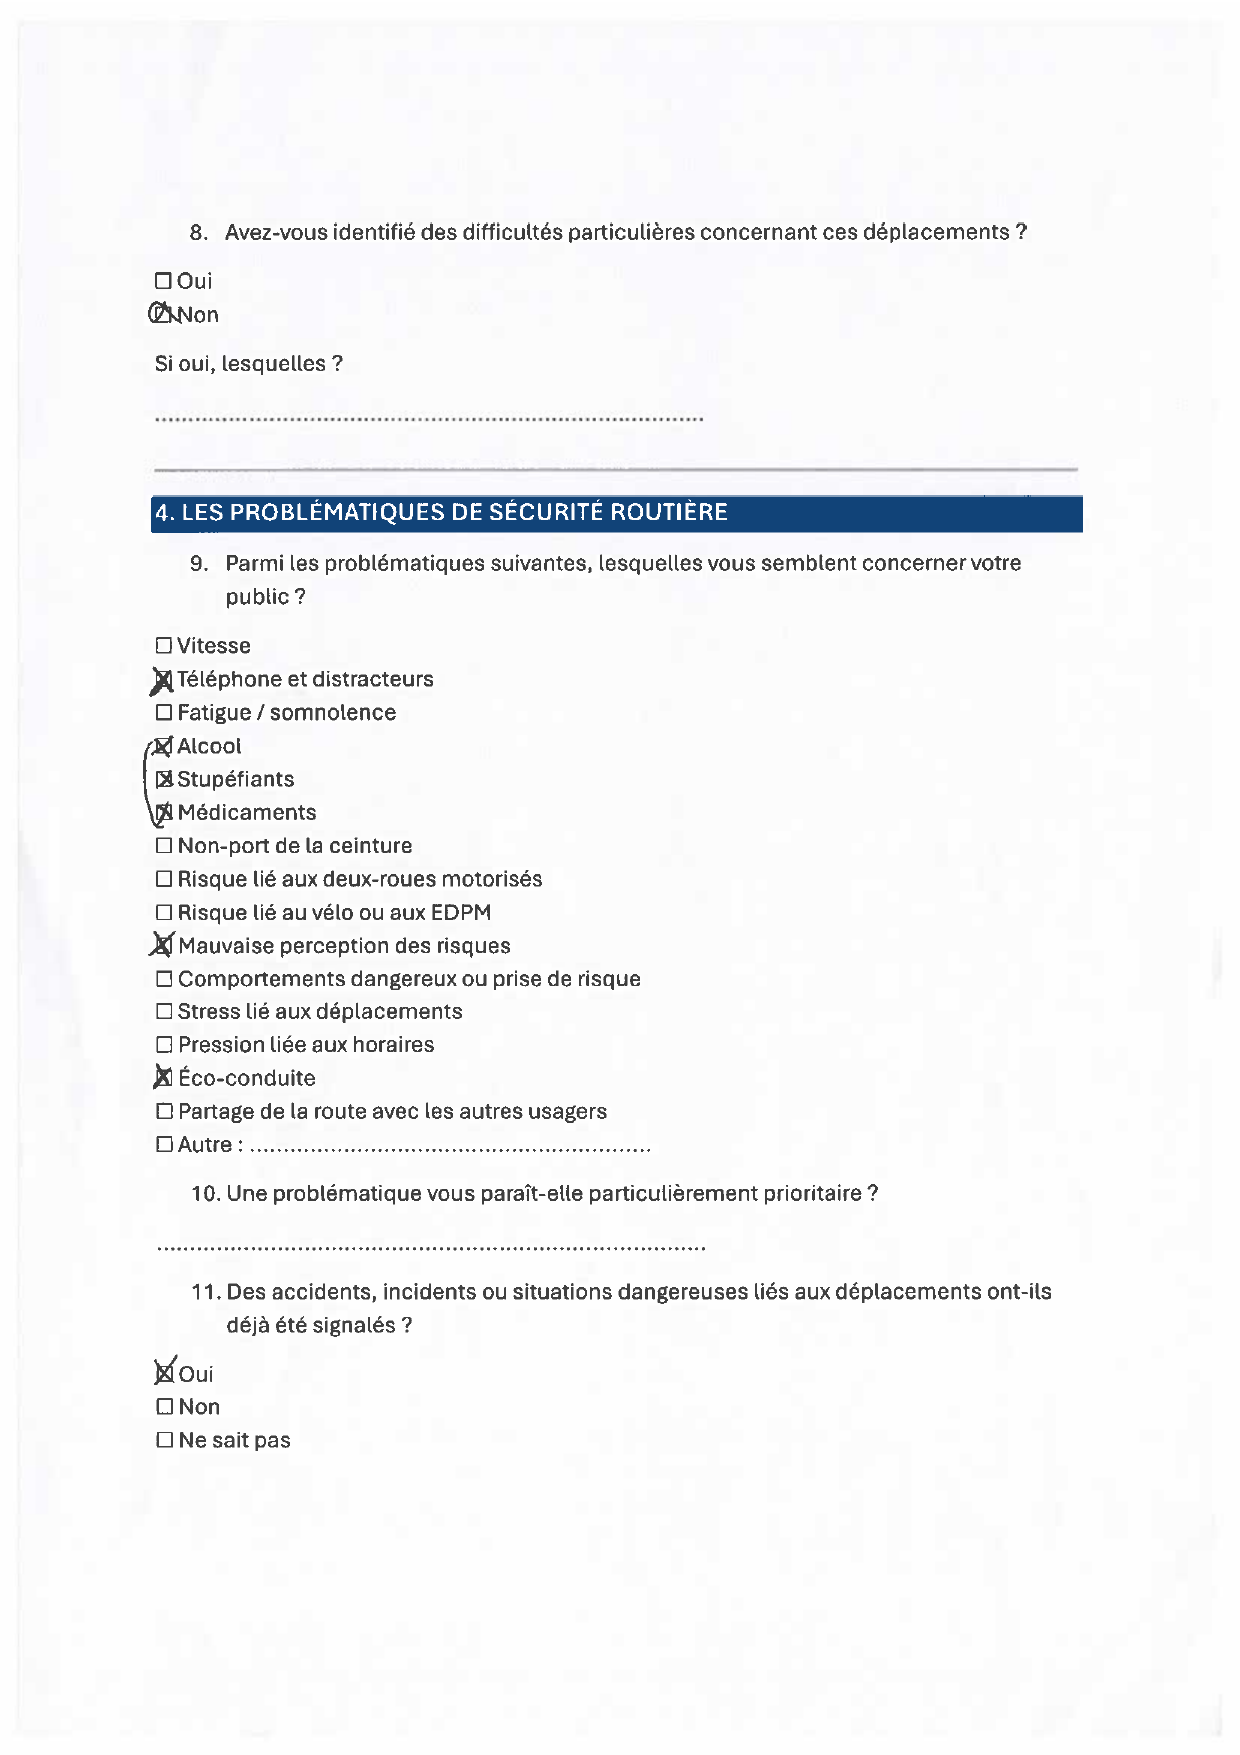
\includegraphics[width=0.92\textwidth]{images/annexes/questionnaire_commanditaire-3.png}
\end{figure}

\clearpage
\subsection*{Questionnaire commanditaire --- page 4}
\begin{figure}[H]
\centering
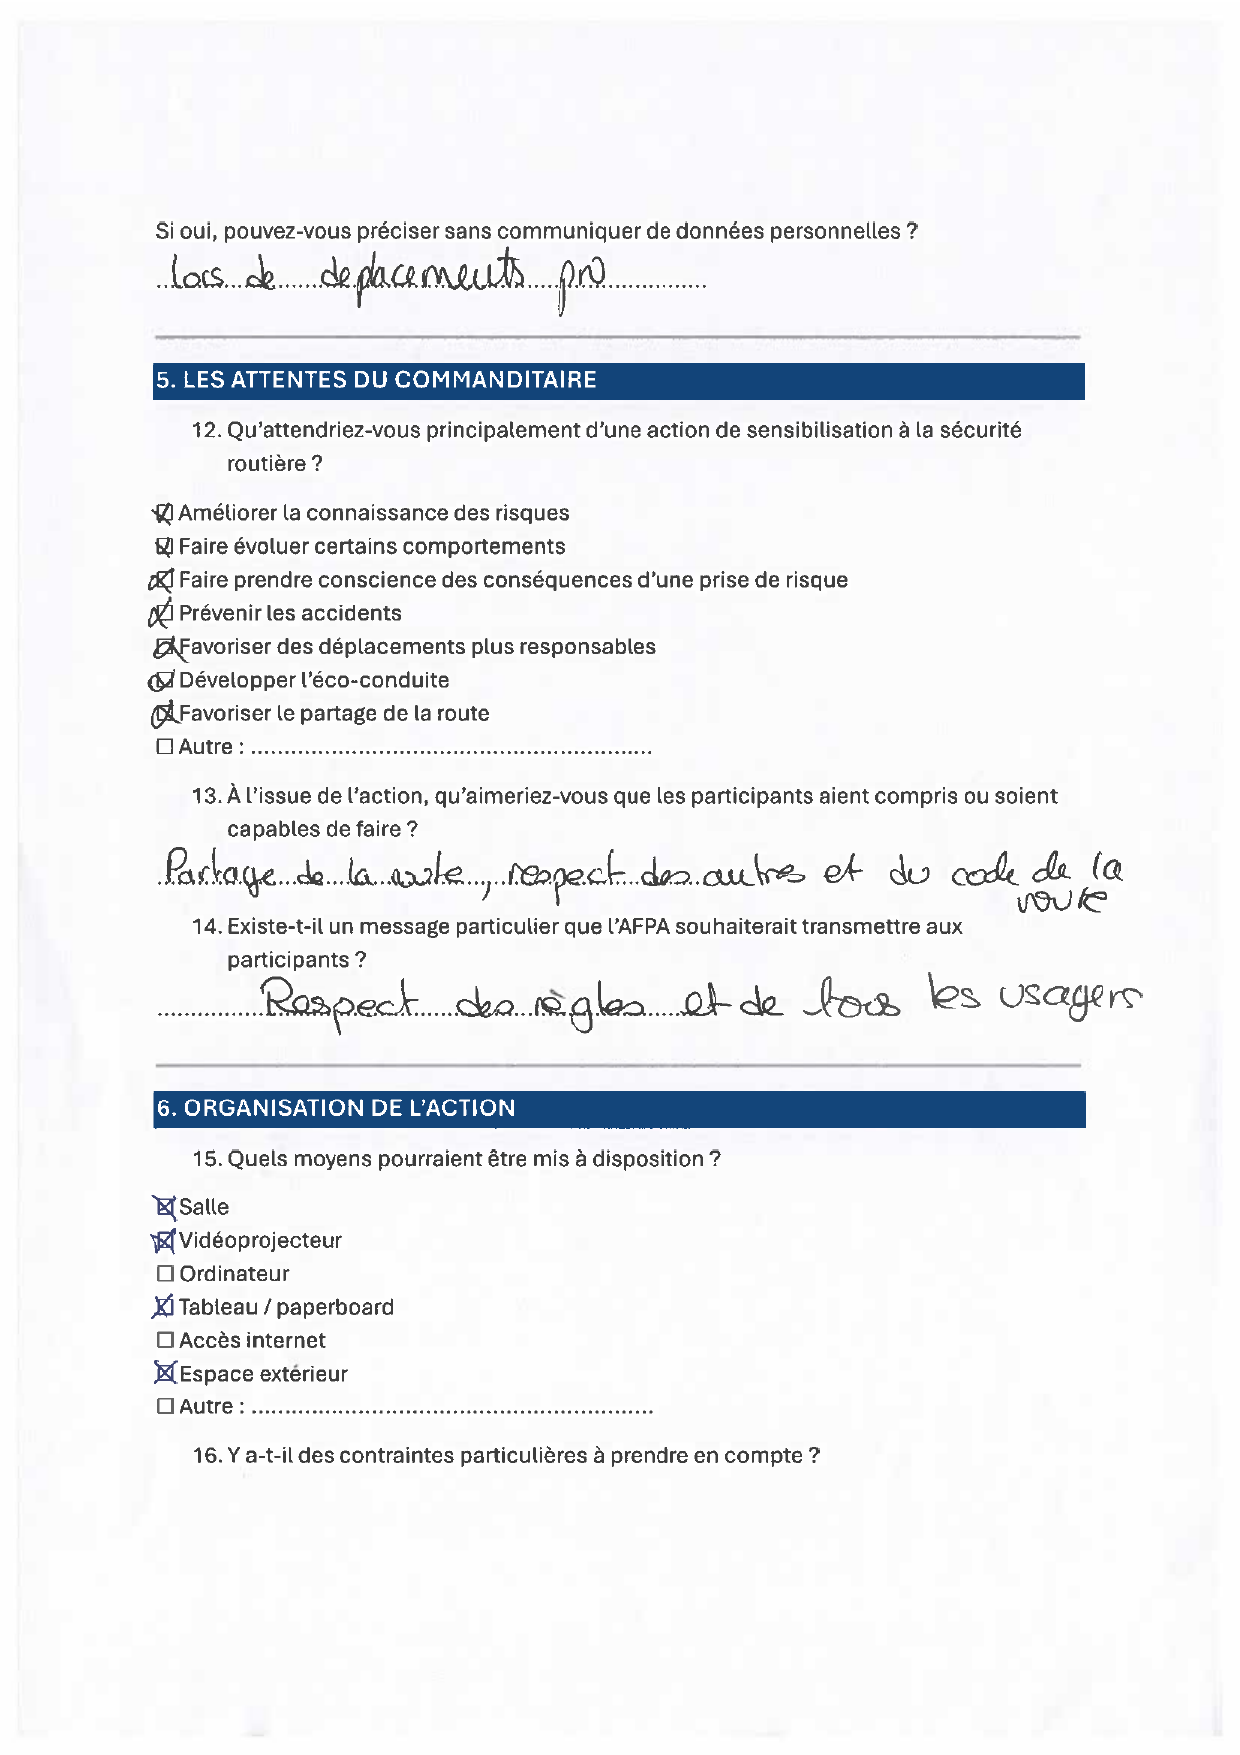
\includegraphics[width=0.92\textwidth]{images/annexes/questionnaire_commanditaire-4.png}
\end{figure}

\clearpage
\subsection*{Questionnaire commanditaire --- page 5}
\begin{figure}[H]
\centering
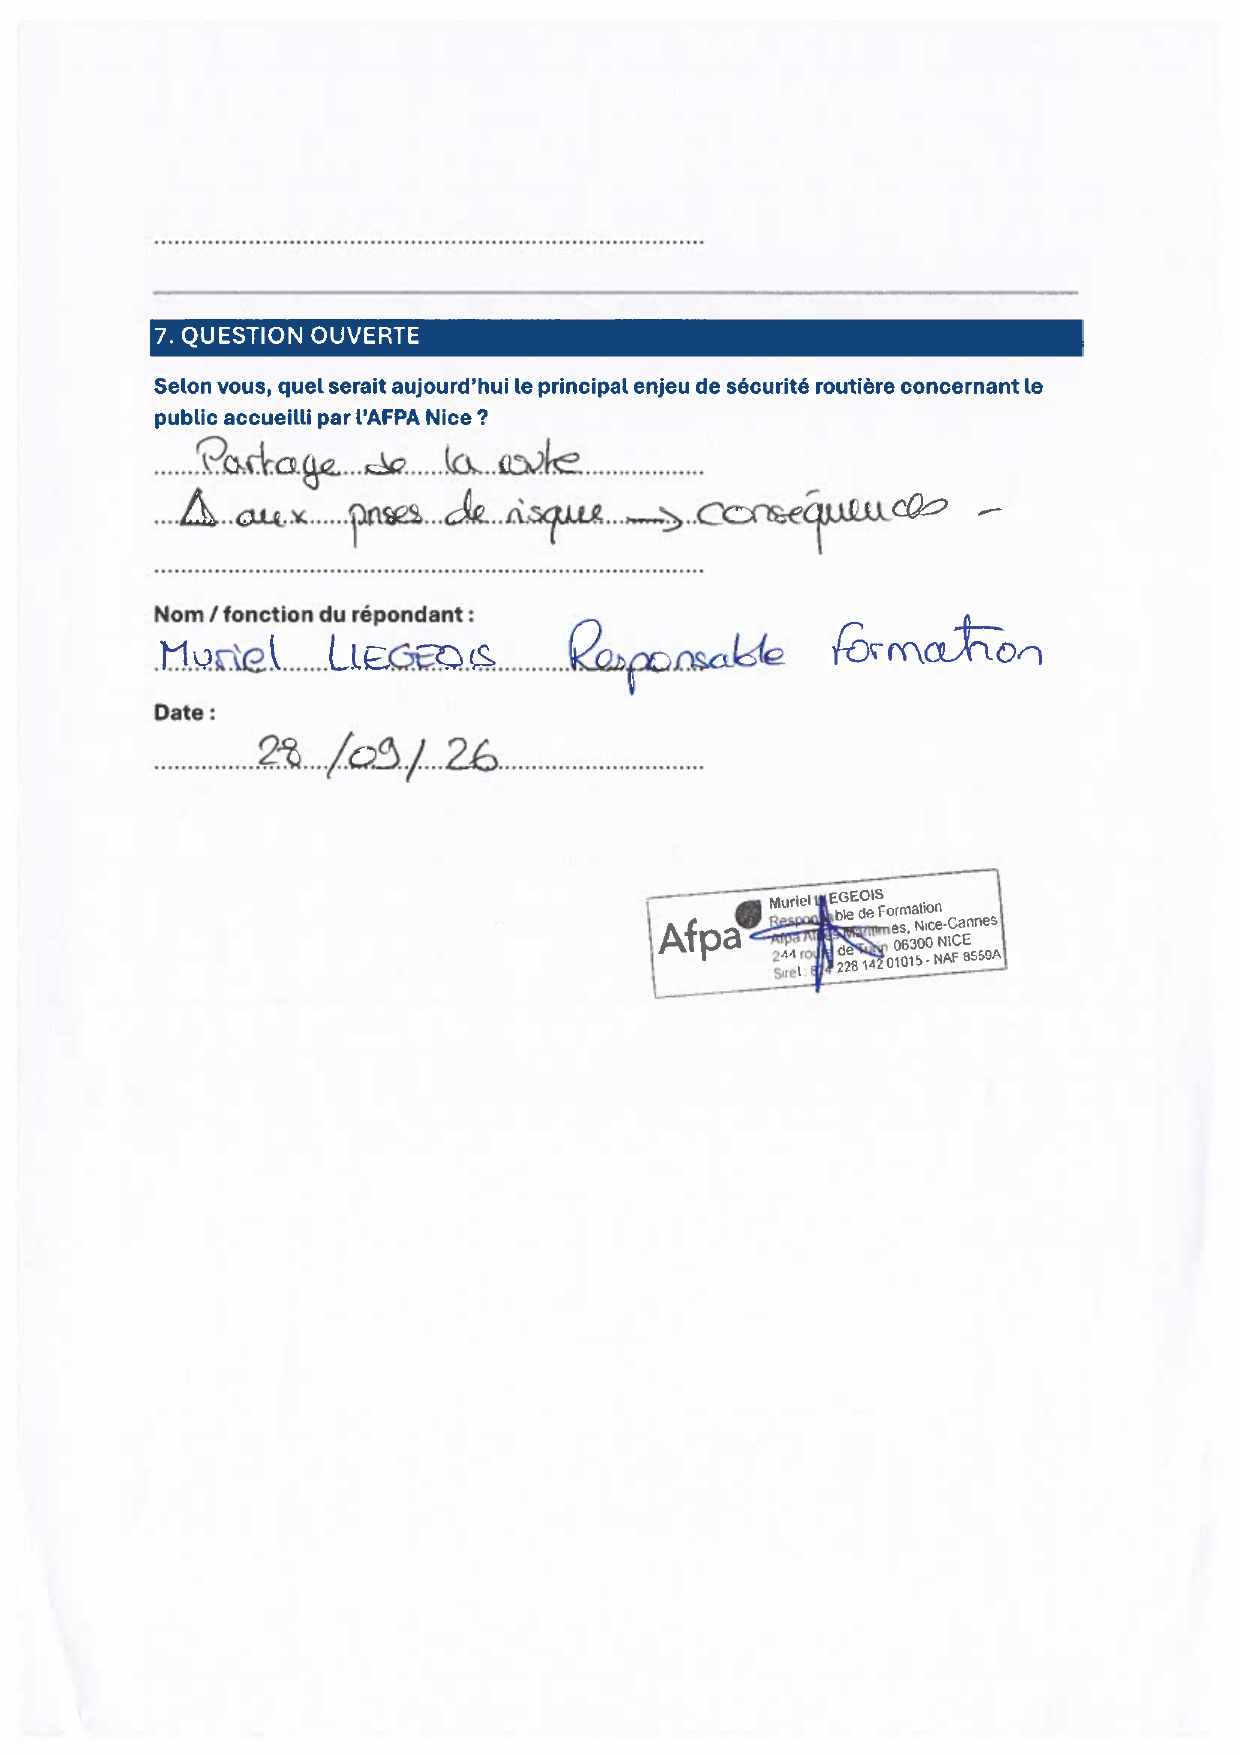
\includegraphics[width=0.92\textwidth]{images/annexes/questionnaire_commanditaire-5.png}
\end{figure}

\section{Échanges sur la clarification et le rendez-vous (A3)}
Ces pièces montrent les échanges autour de la réponse du commanditaire, de la date d’intervention et du rendez-vous du 1er octobre.

\clearpage
\begin{landscape}
\thispagestyle{plain}
\noindent{\large\bfseries 28 septembre — Retour annoncé et proposition d’intervention}\par\medskip
\begin{center}
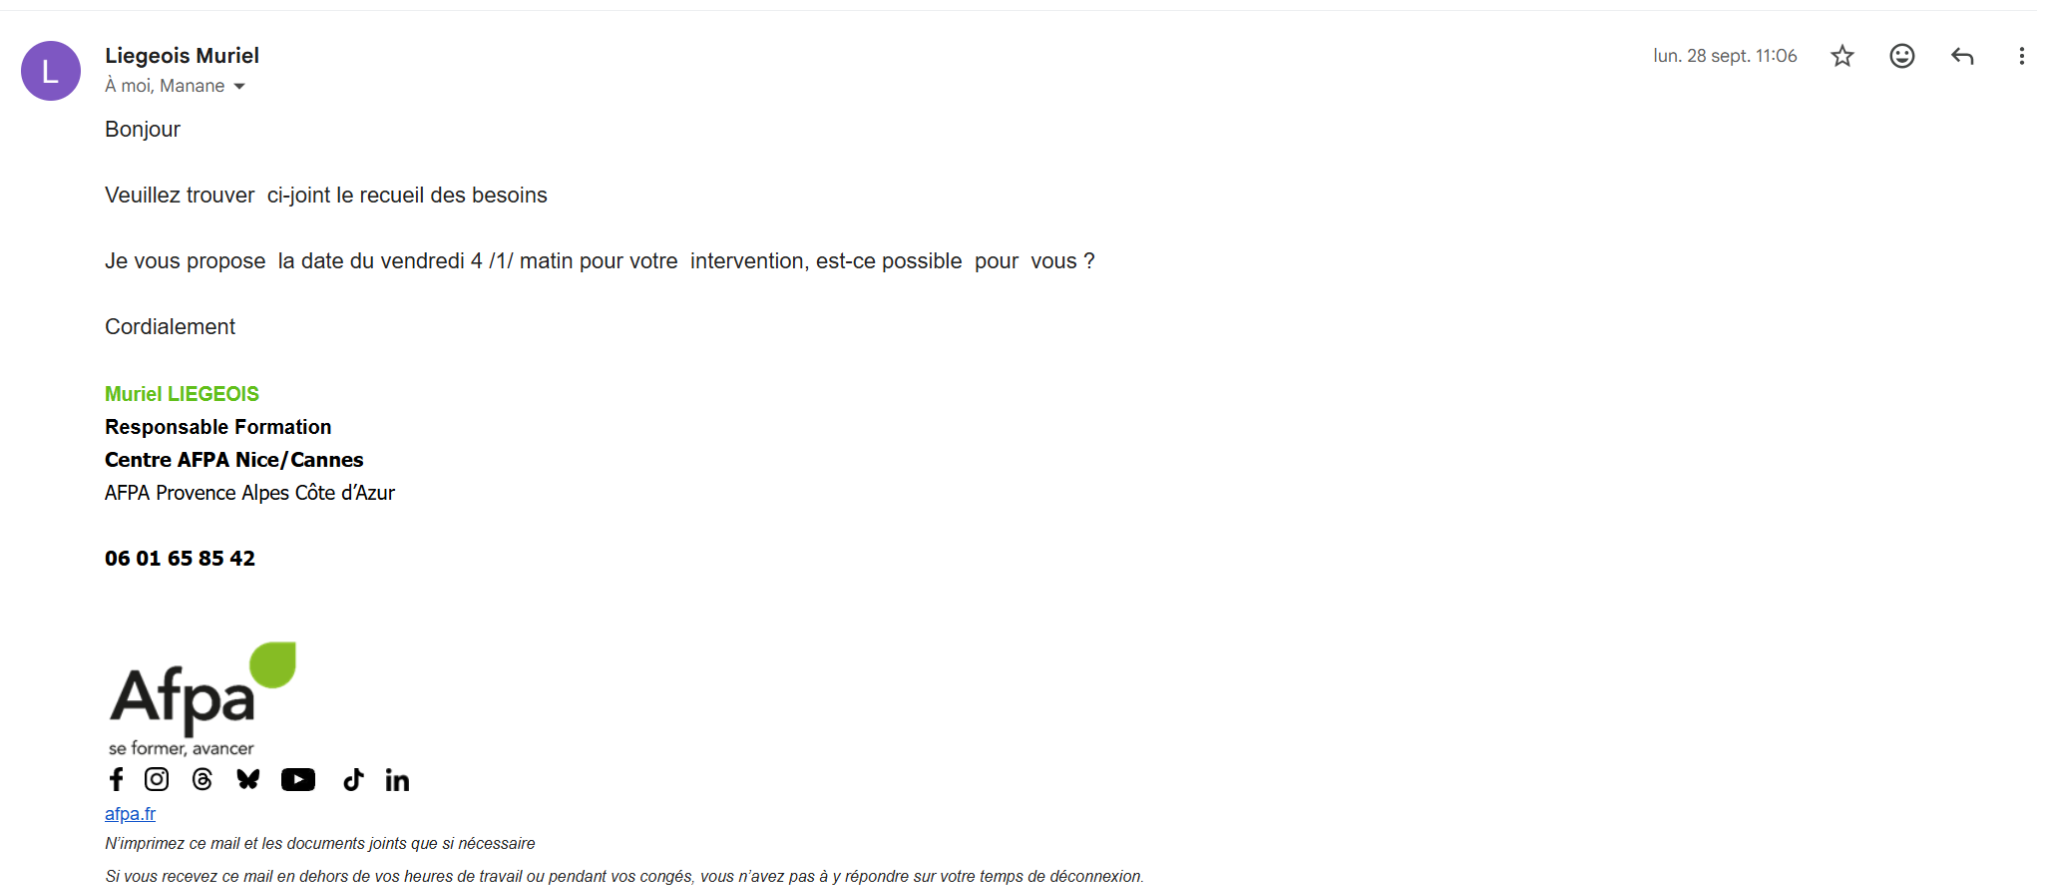
\includegraphics[width=0.97\linewidth,height=0.77\textheight,keepaspectratio]{images/annexes/echanges/a06_20260928_reponse_afpa.png}
\end{center}
\end{landscape}

\clearpage
\begin{landscape}
\thispagestyle{plain}
\noindent{\large\bfseries 28 septembre — Demande d’entretien complémentaire}\par\medskip
\begin{center}
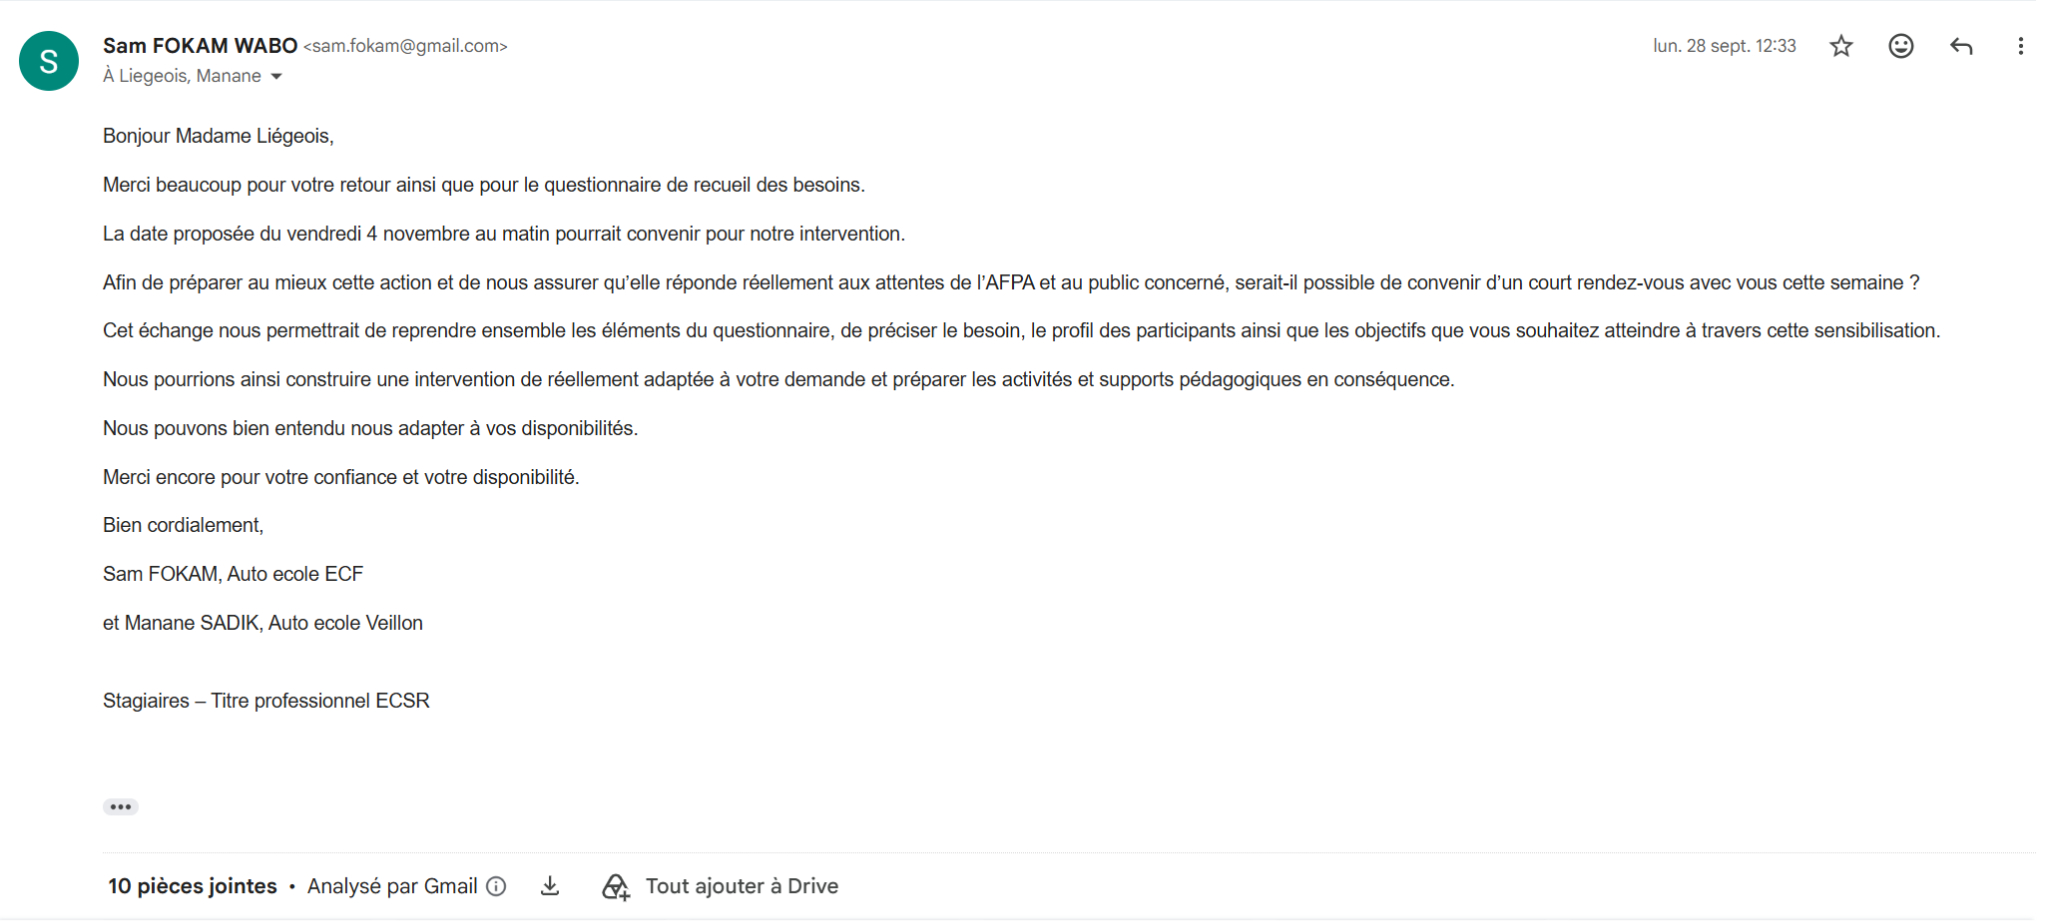
\includegraphics[width=0.97\linewidth,height=0.77\textheight,keepaspectratio]{images/annexes/echanges/a07_20260928_demande_rdv.png}
\end{center}
\end{landscape}

\clearpage
\begin{landscape}
\thispagestyle{plain}
\noindent{\large\bfseries 28 septembre — Rectification de la date et proposition de rendez-vous}\par\medskip
\begin{center}
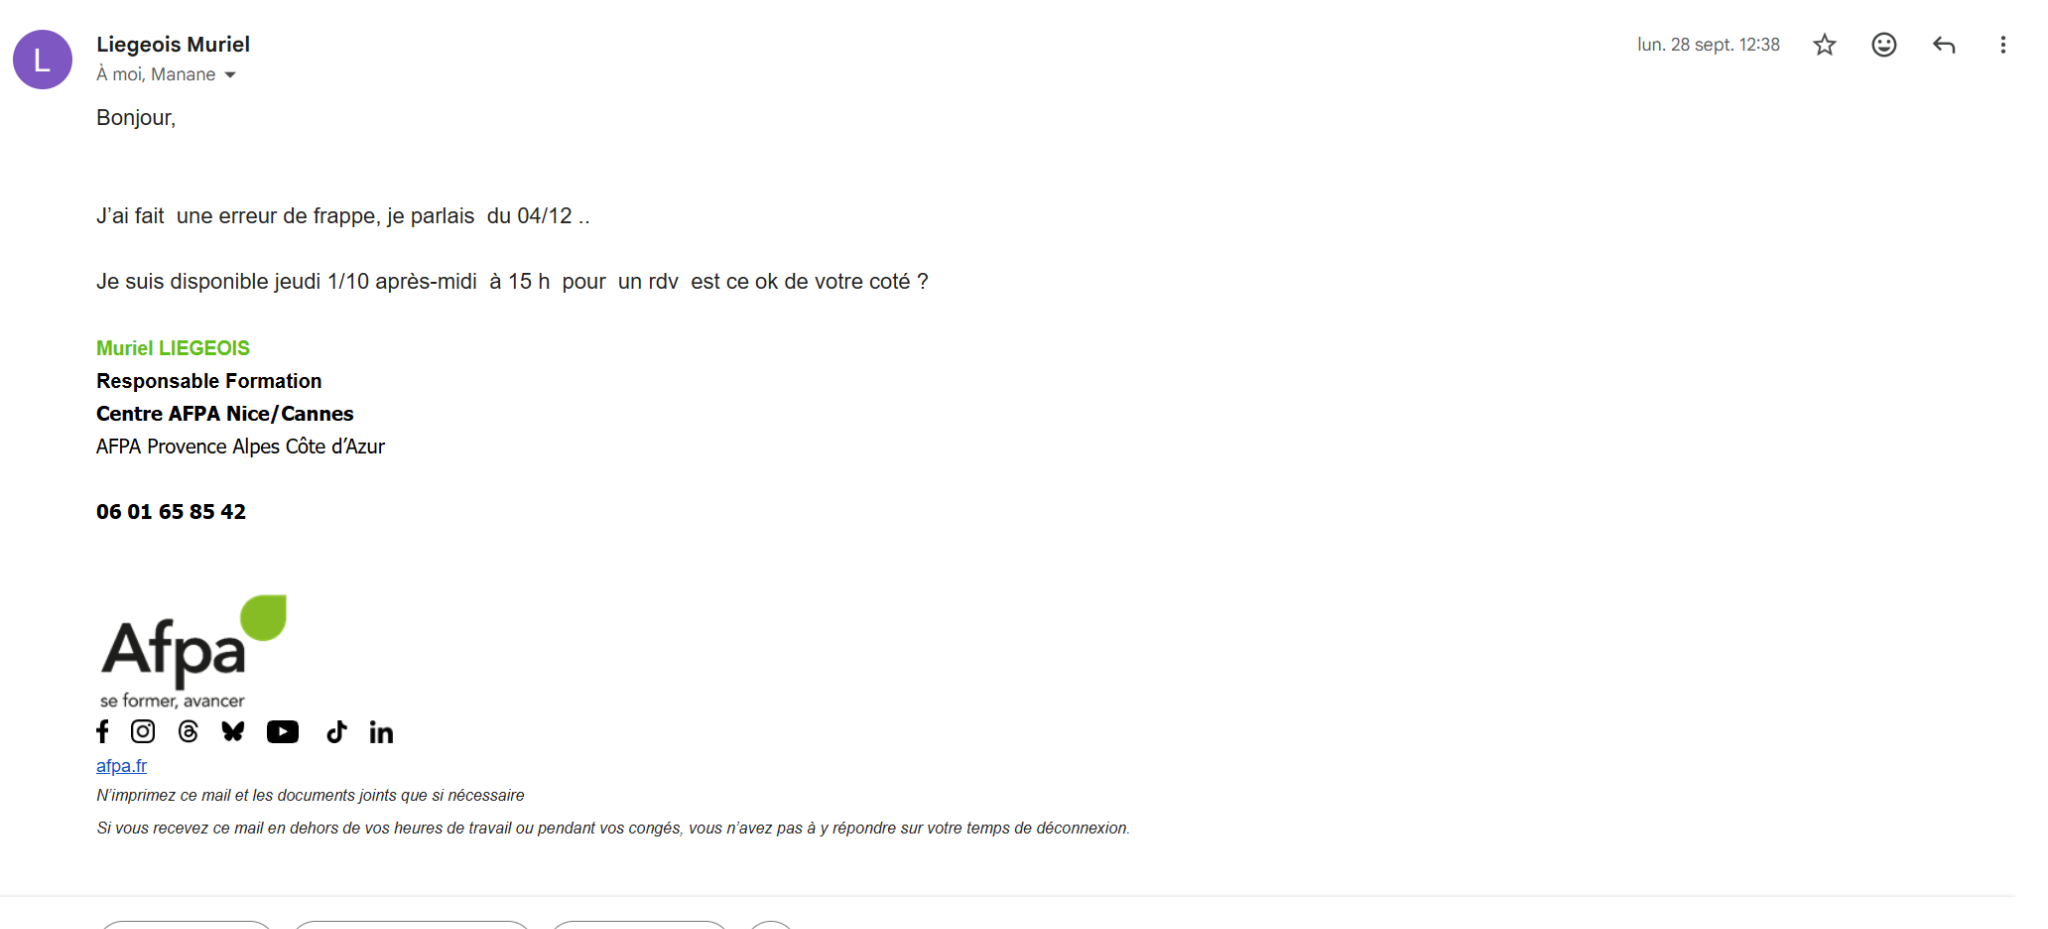
\includegraphics[width=0.97\linewidth,height=0.77\textheight,keepaspectratio]{images/annexes/echanges/a08_20260928_date_et_rdv.png}
\end{center}
\end{landscape}

\clearpage
\begin{landscape}
\thispagestyle{plain}
\noindent{\large\bfseries 28 septembre — Confirmation du rendez-vous}\par\medskip
\begin{center}

\includegraphics[width=0.97\linewidth,height=0.77\textheight,keepaspectratio]{images/annexes/echanges/a09_20260928_confirmation.png}
\end{center}
\end{landscape}

\clearpage
\begin{landscape}
\thispagestyle{plain}
\noindent{\large\bfseries 28 septembre — Invitation Outlook confirmée}\par\medskip
\begin{center}
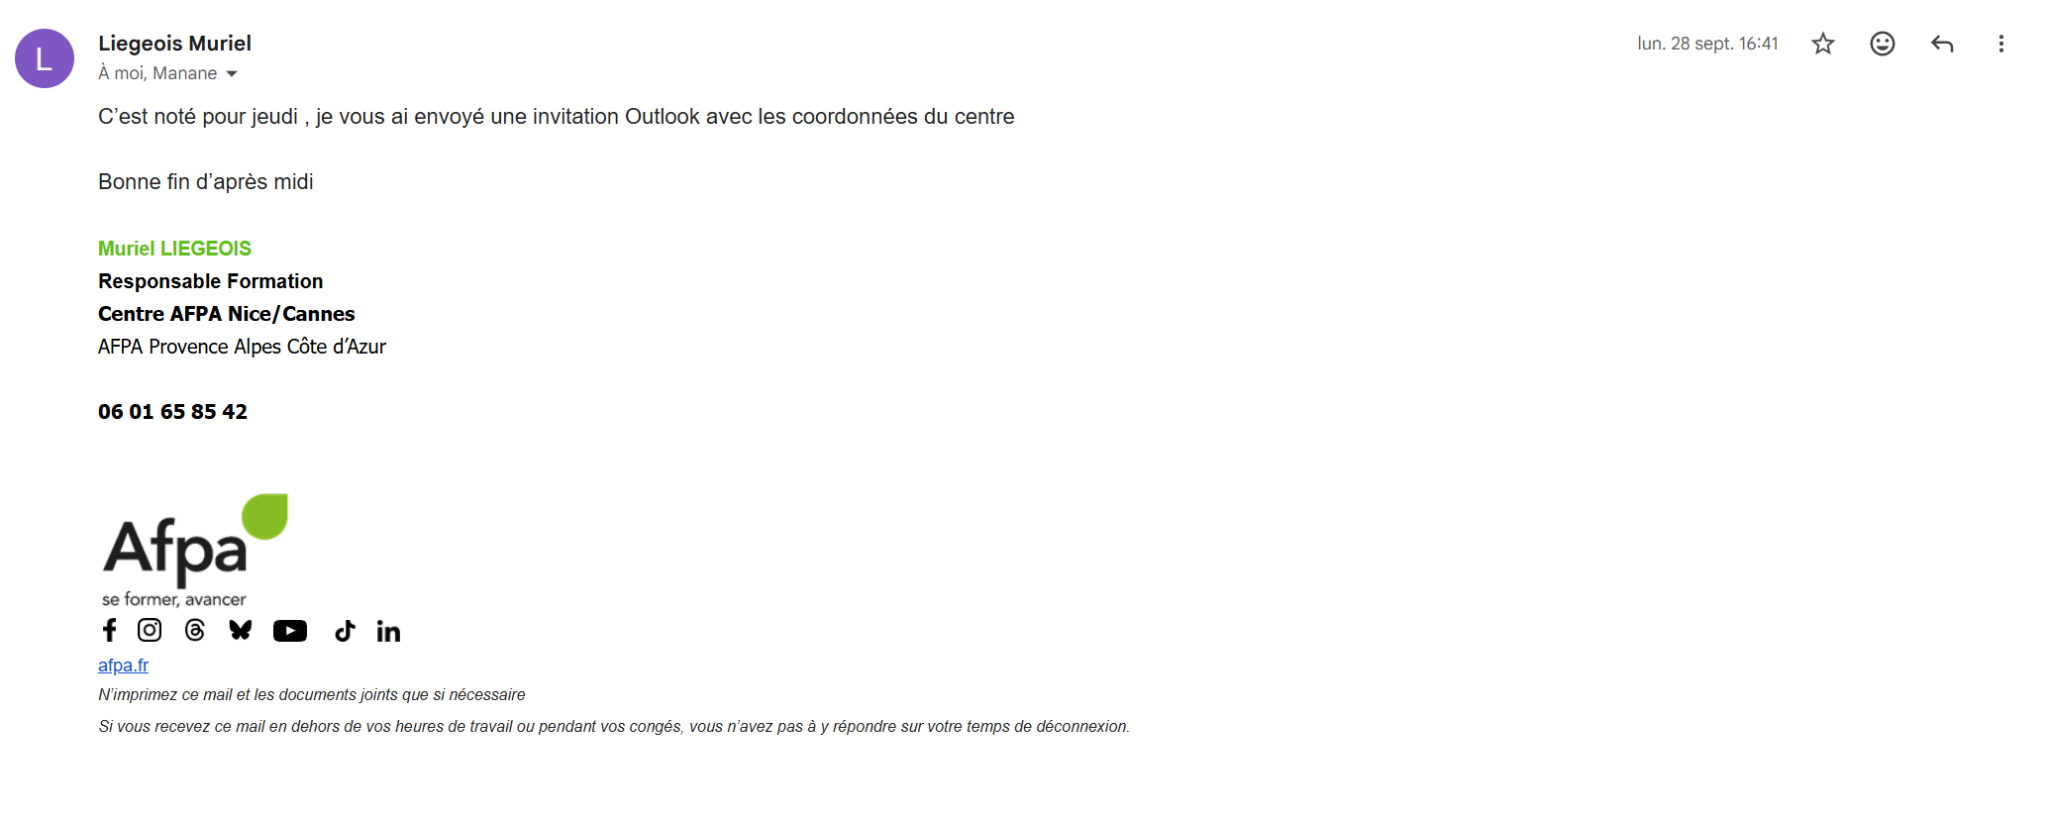
\includegraphics[width=0.97\linewidth,height=0.77\textheight,keepaspectratio]{images/annexes/echanges/a10_20260928_invitation.png}
\end{center}
\end{landscape}

\clearpage
\begin{landscape}
\thispagestyle{plain}
\noindent{\large\bfseries 28 septembre — Nouvelle demande de la pièce jointe}\par\medskip
\begin{center}
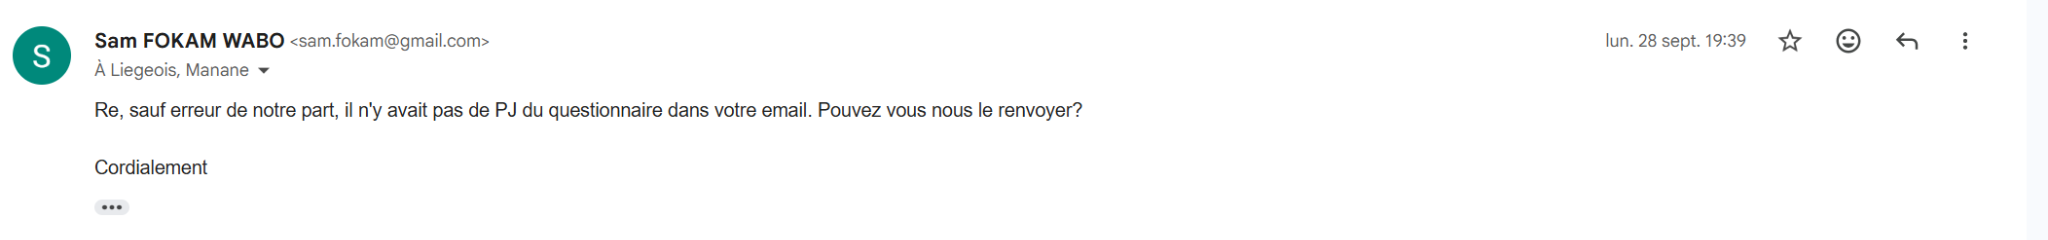
\includegraphics[width=0.97\linewidth,height=0.77\textheight,keepaspectratio]{images/annexes/echanges/a11_20260928_pj_absente.png}
\end{center}
\end{landscape}

\clearpage
\begin{landscape}
\thispagestyle{plain}
\noindent{\large\bfseries 29 septembre — Envoi effectif des réponses du commanditaire}\par\medskip
\begin{center}
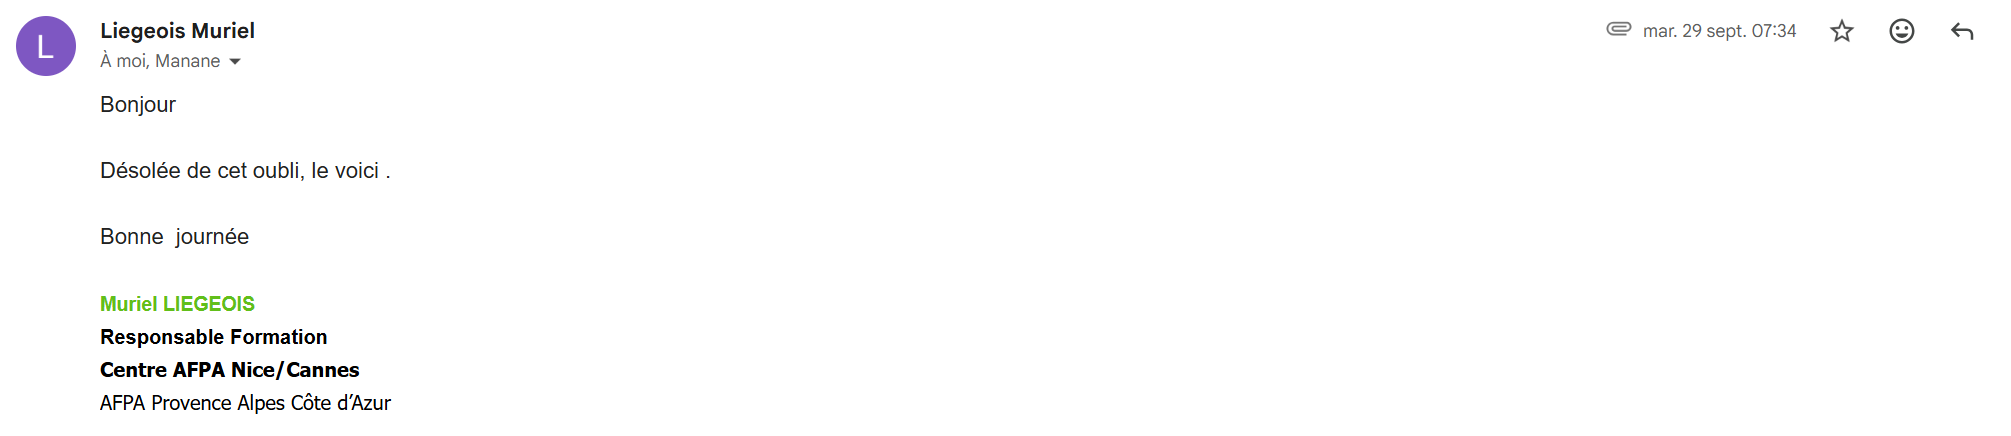
\includegraphics[width=0.97\linewidth,height=0.77\textheight,keepaspectratio]{images/annexes/echanges/a12_20260929_questionnaire_recu.png}
\end{center}
\end{landscape}

\section{Questionnaire destiné aux stagiaires (A4)}
Les pages suivantes reproduisent, sous forme d'images, le questionnaire anonyme de trente questions destiné aux stagiaires plombiers de l'AFPA. Cette pièce correspond à la partie consacrée au diagnostic du public et à l'identification du besoin réel.

\clearpage
\subsection*{Questionnaire stagiaires --- page 1}
\begin{figure}[H]
\centering
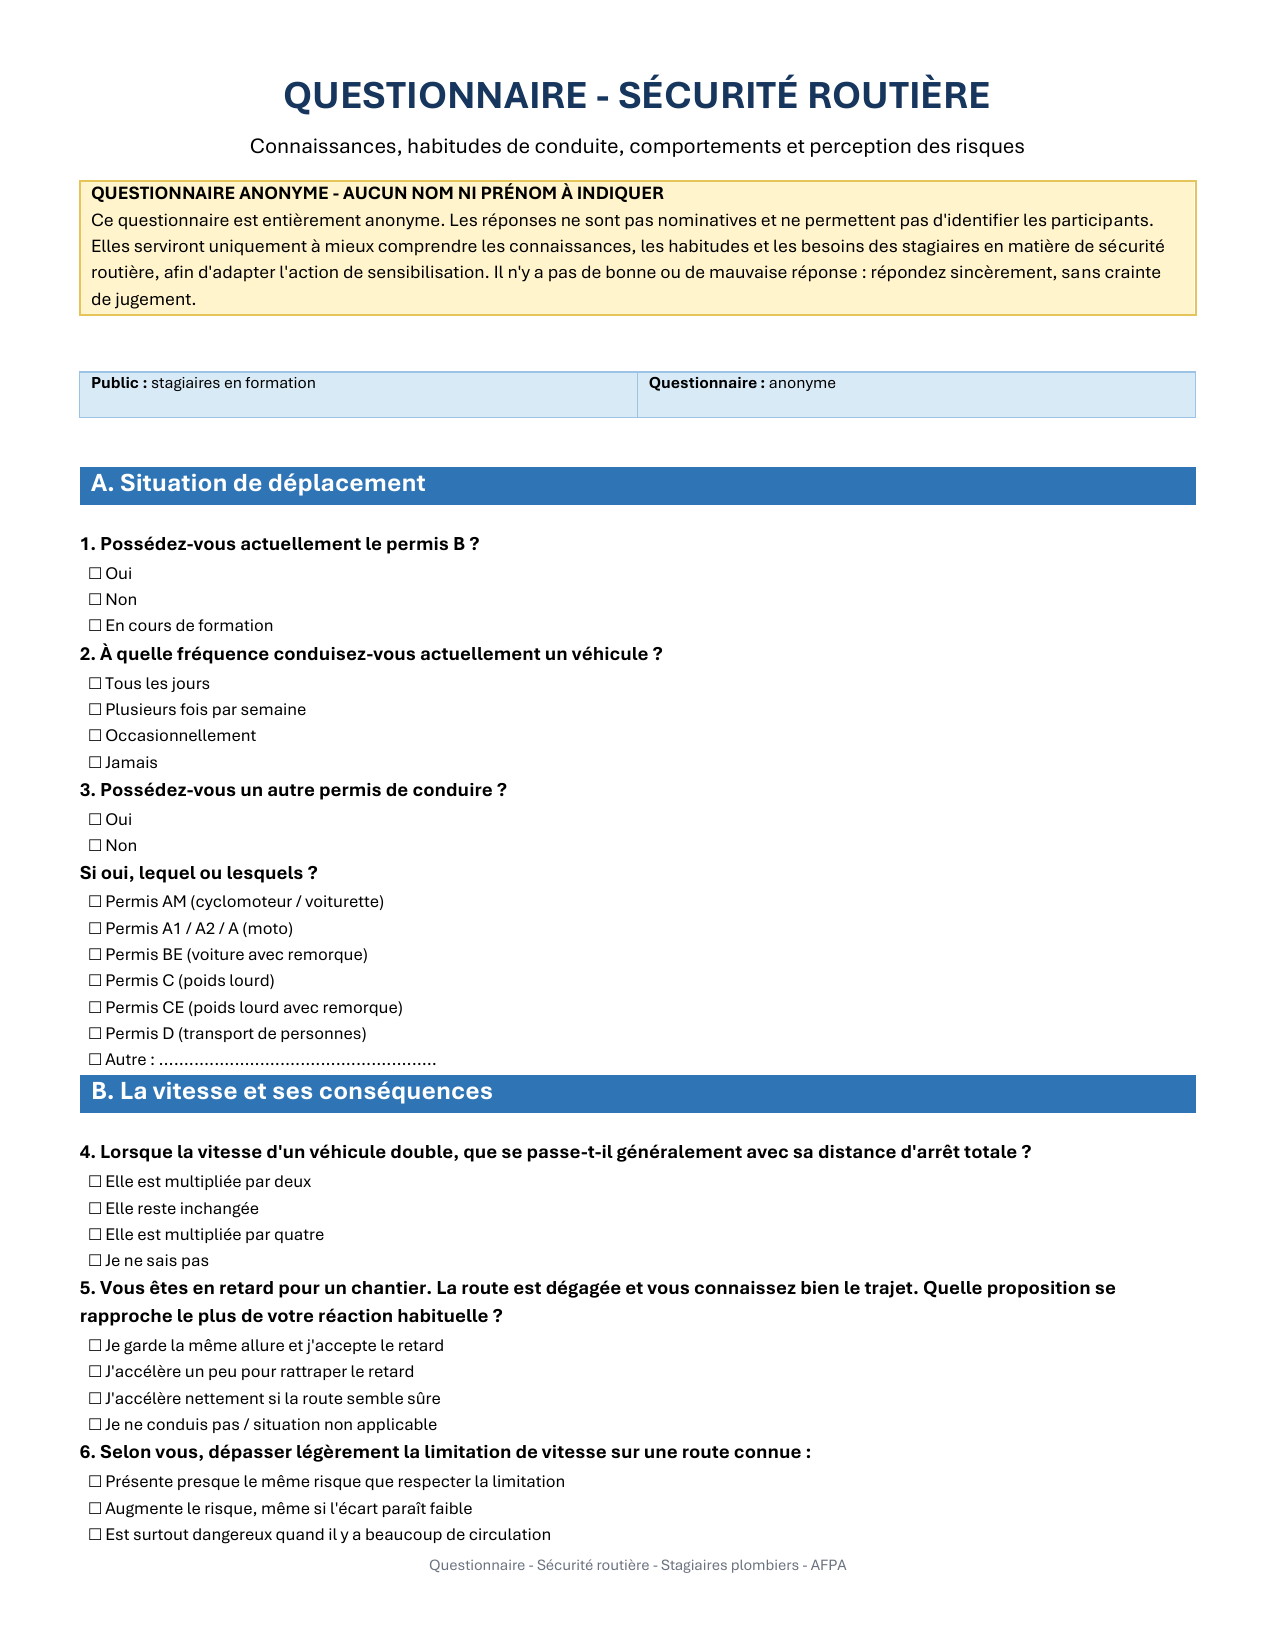
\includegraphics[width=0.92\textwidth]{images/annexes/questionnaire_stagiaires-1.png}
\end{figure}

\clearpage
\subsection*{Questionnaire stagiaires --- page 2}
\begin{figure}[H]
\centering
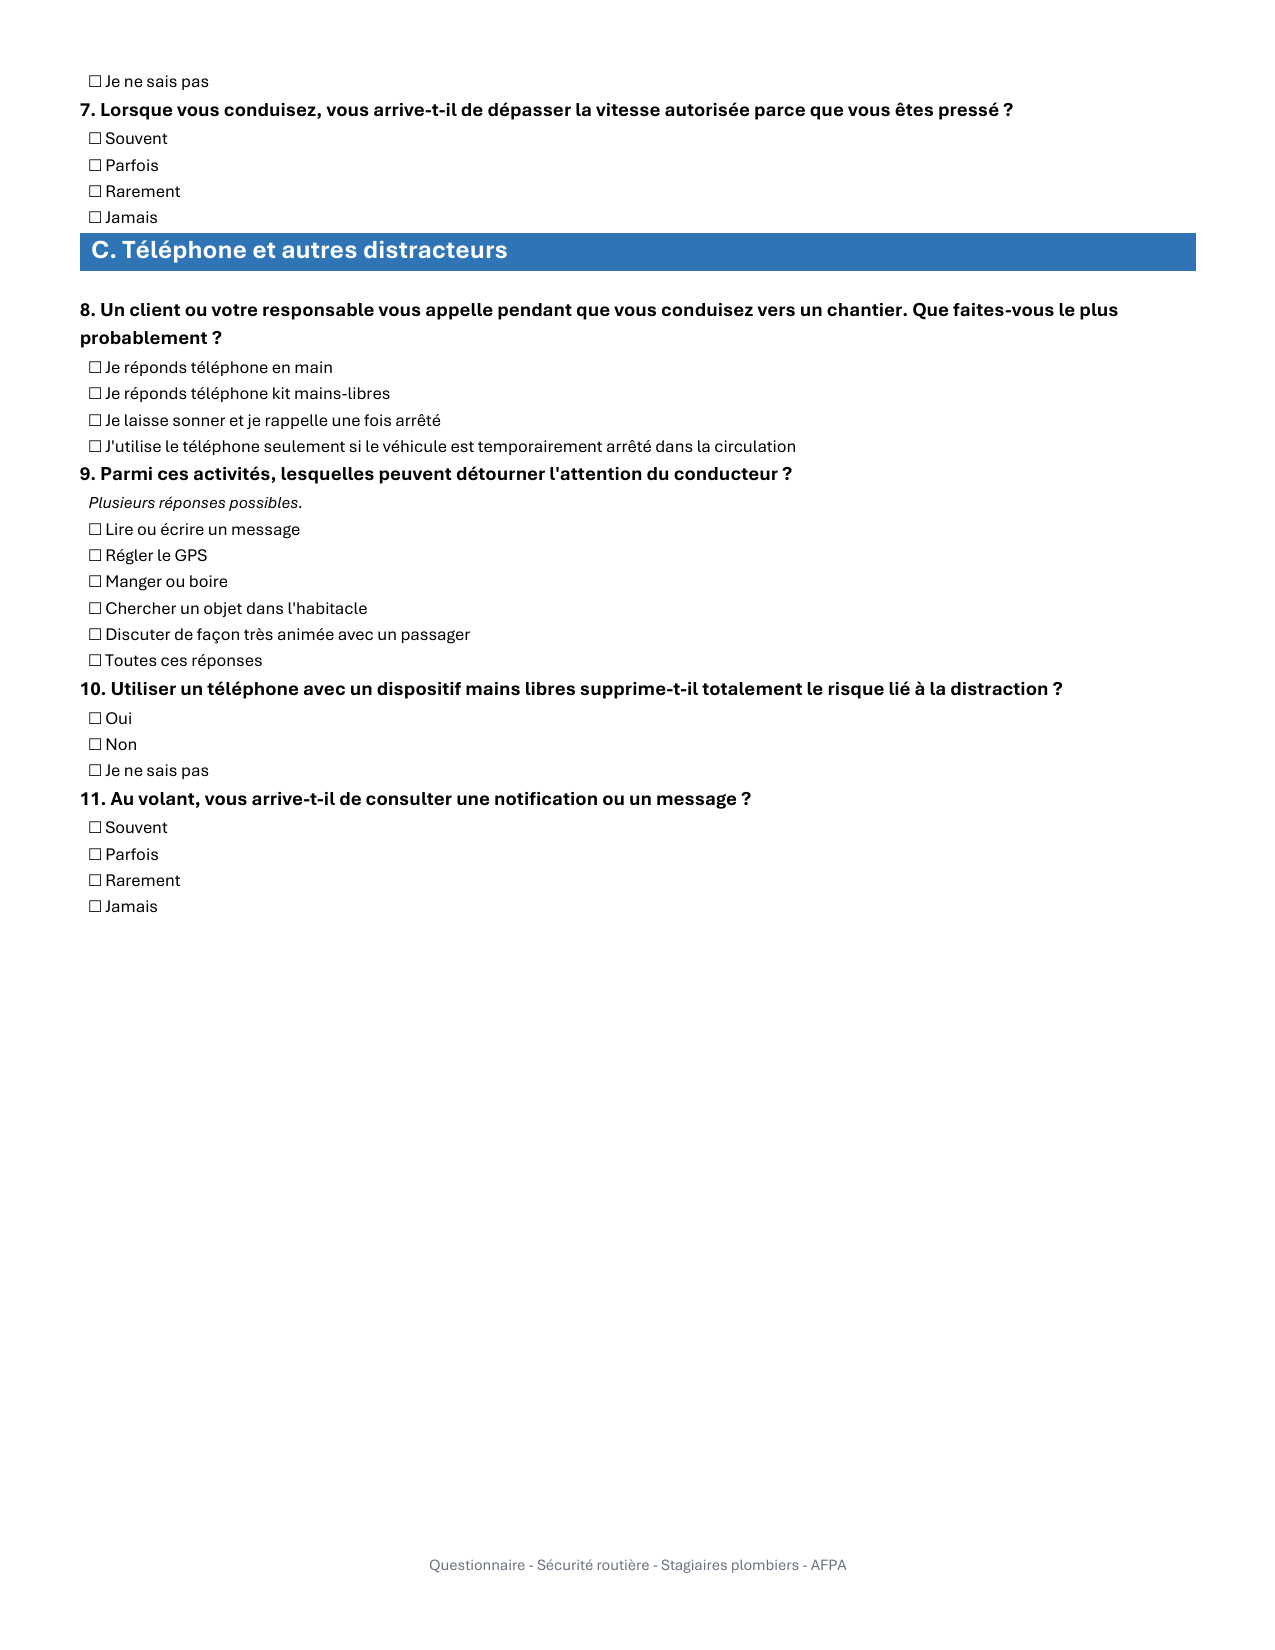
\includegraphics[width=0.92\textwidth]{images/annexes/questionnaire_stagiaires-2.png}
\end{figure}

\clearpage
\subsection*{Questionnaire stagiaires --- page 3}
\begin{figure}[H]
\centering
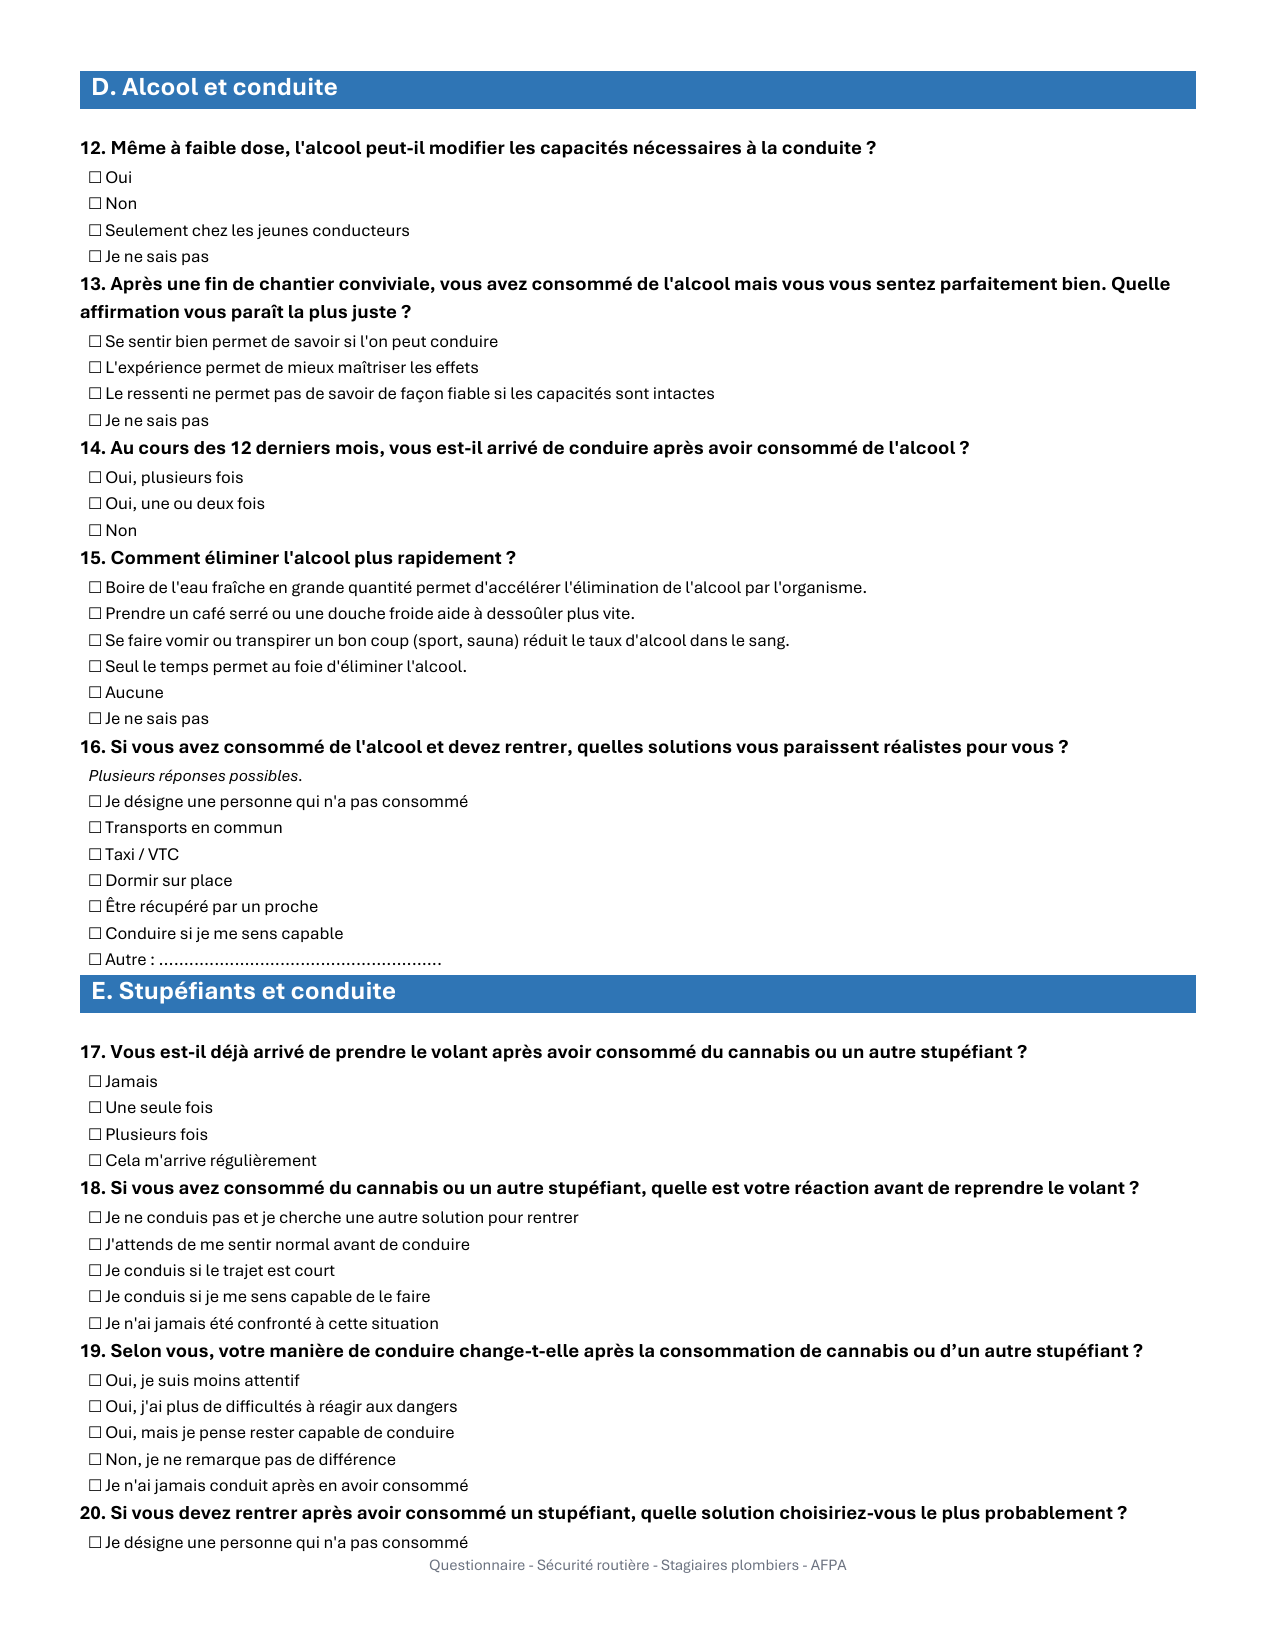
\includegraphics[width=0.92\textwidth]{images/annexes/questionnaire_stagiaires-3.png}
\end{figure}

\clearpage
\subsection*{Questionnaire stagiaires --- page 4}
\begin{figure}[H]
\centering
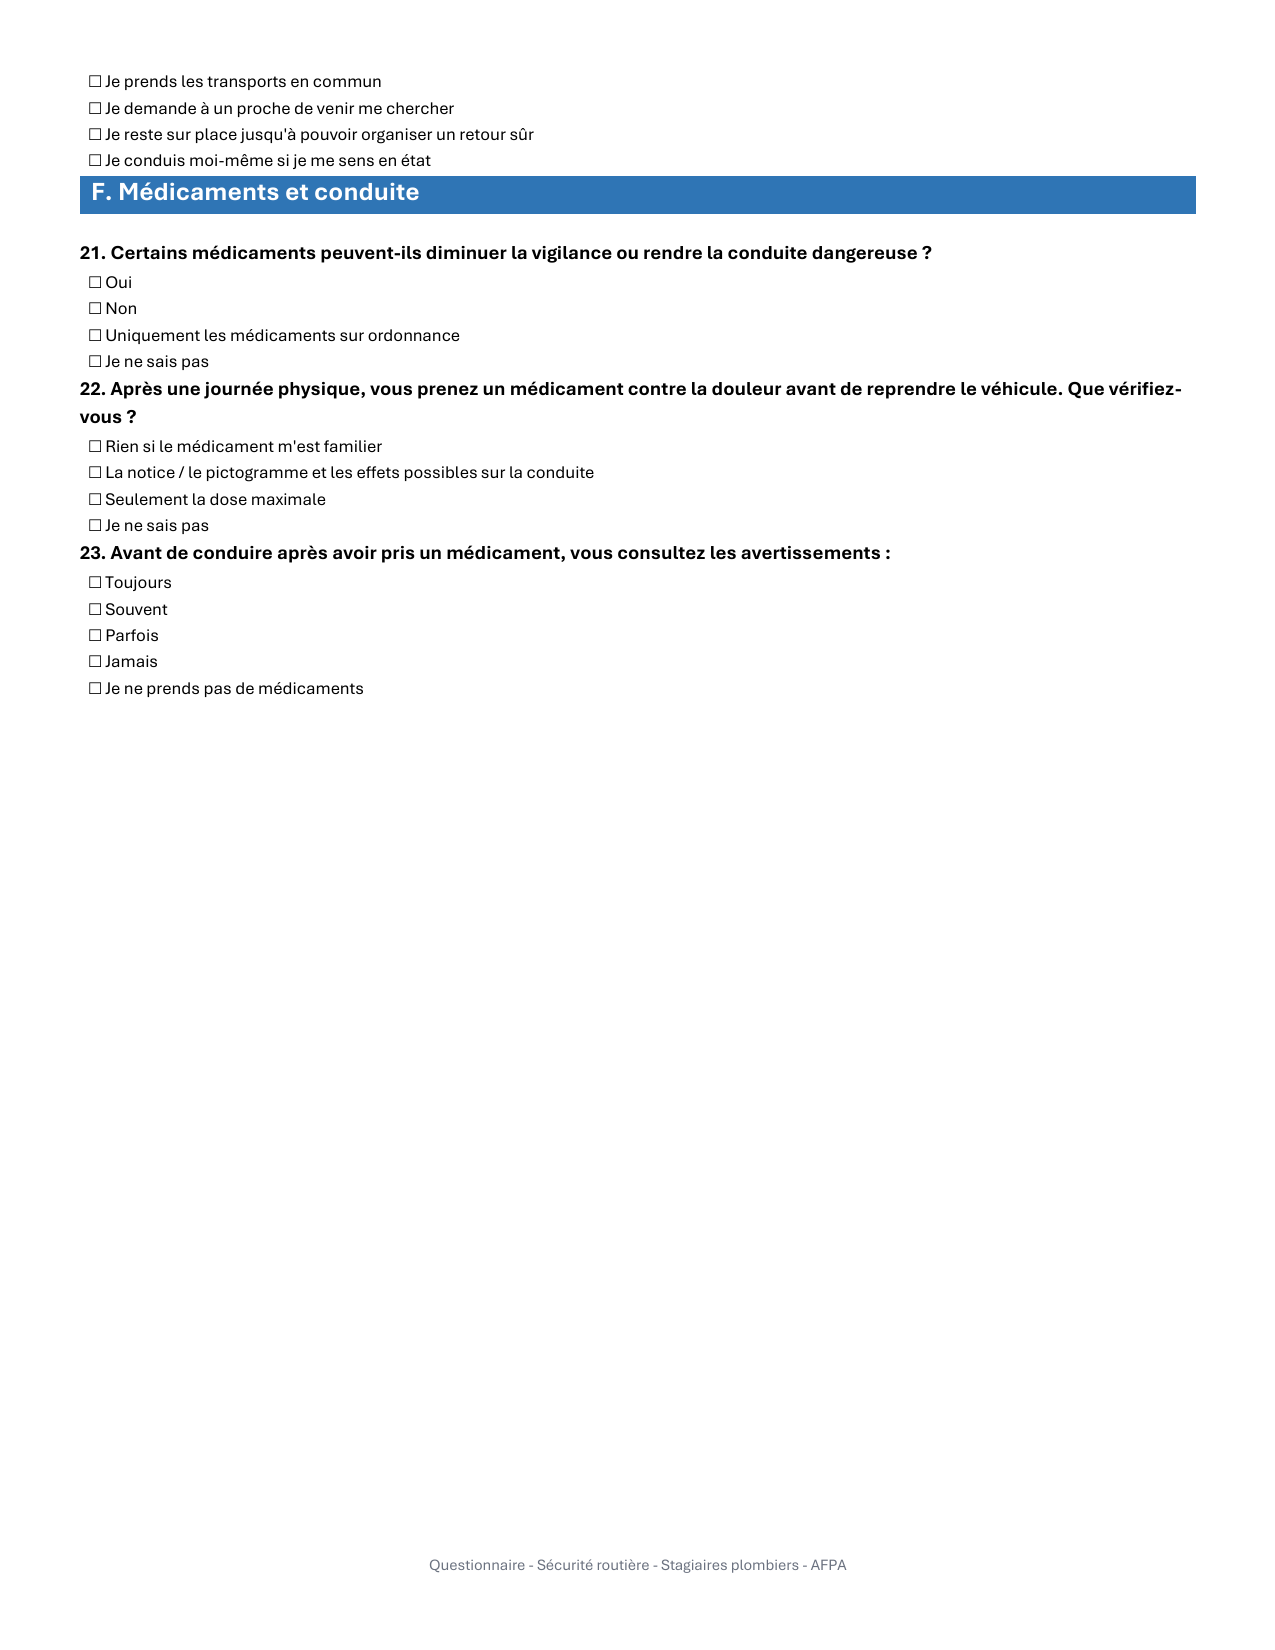
\includegraphics[width=0.92\textwidth]{images/annexes/questionnaire_stagiaires-4.png}
\end{figure}

\clearpage
\subsection*{Questionnaire stagiaires --- page 5}
\begin{figure}[H]
\centering
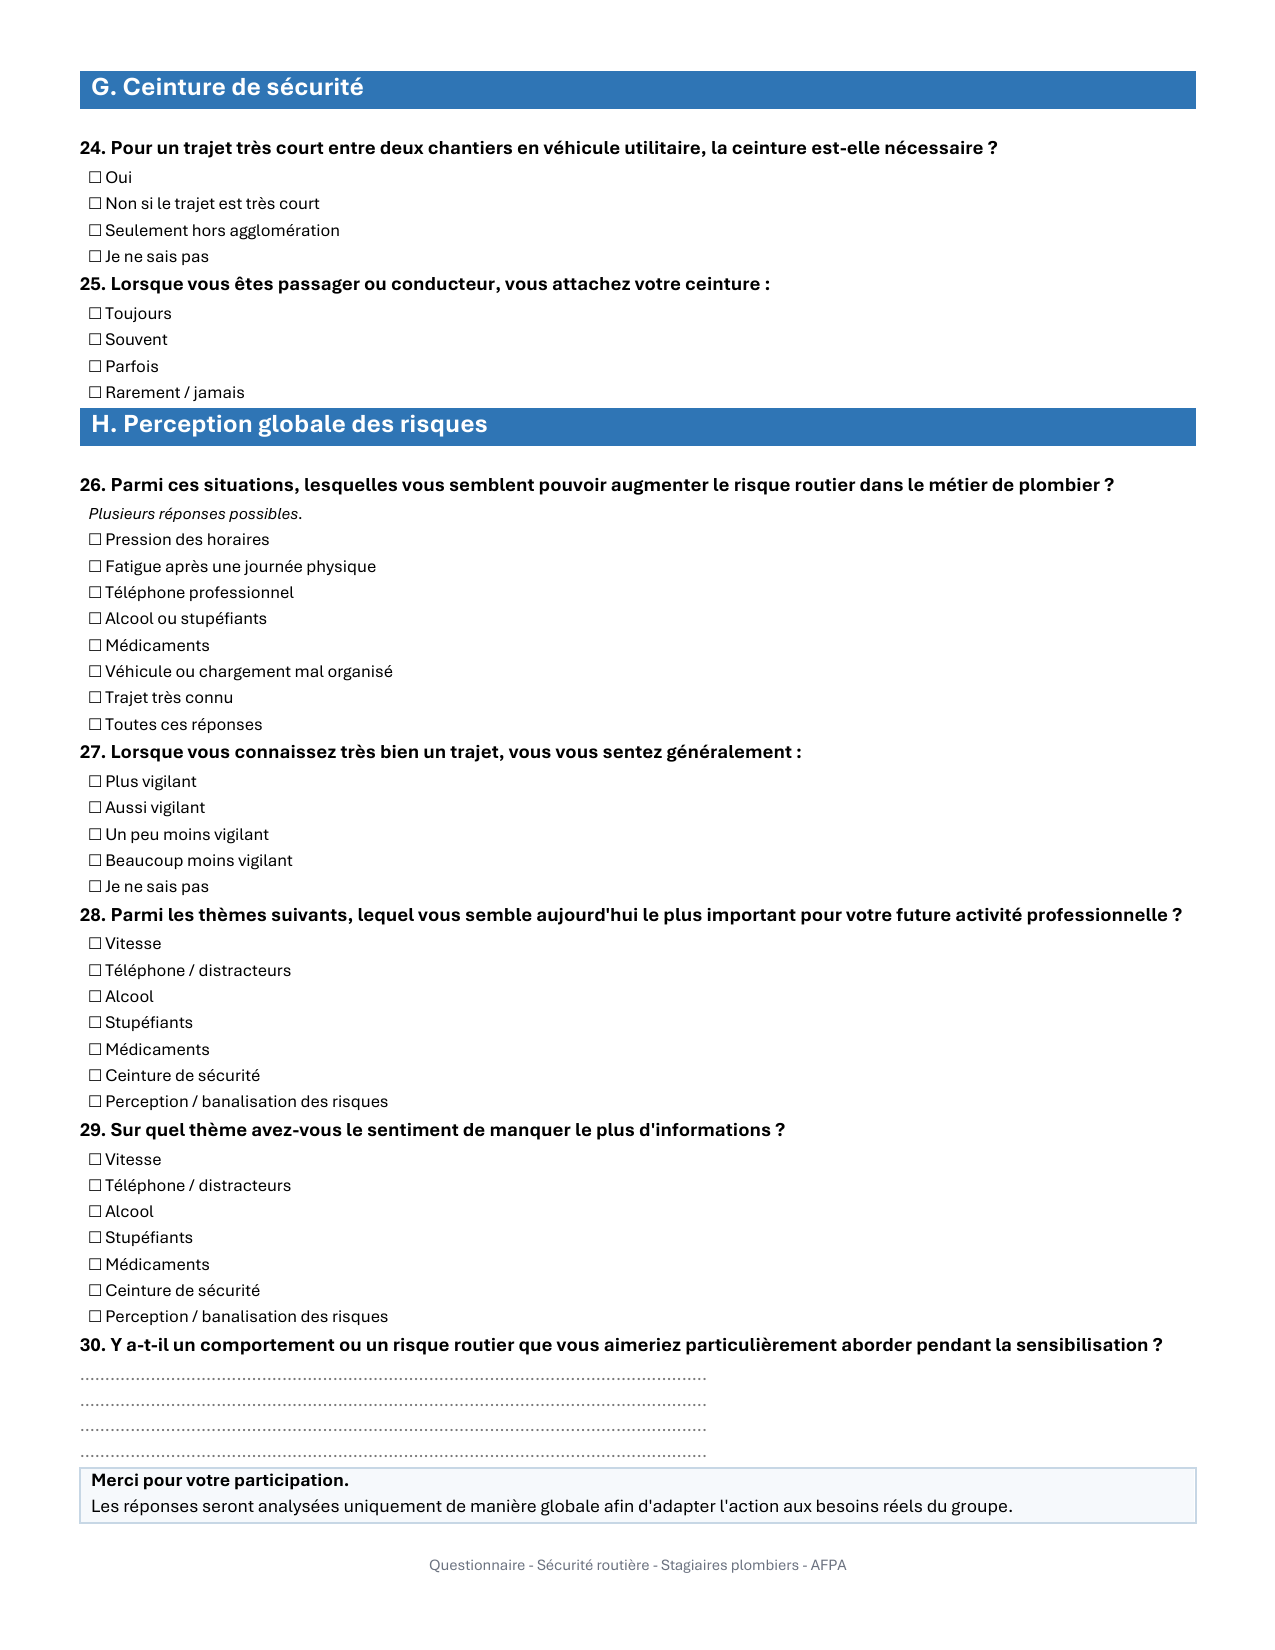
\includegraphics[width=0.92\textwidth]{images/annexes/questionnaire_stagiaires-5.png}
\end{figure}

\section{Échanges relatifs au questionnaire stagiaires (A5)}
Transmission, diffusion et relance du diagnostic auprès du groupe de stagiaires.

\clearpage
\begin{landscape}
\thispagestyle{plain}
\noindent{\large\bfseries 26 octobre — Transmission du questionnaire aux stagiaires}\par\medskip
\begin{center}
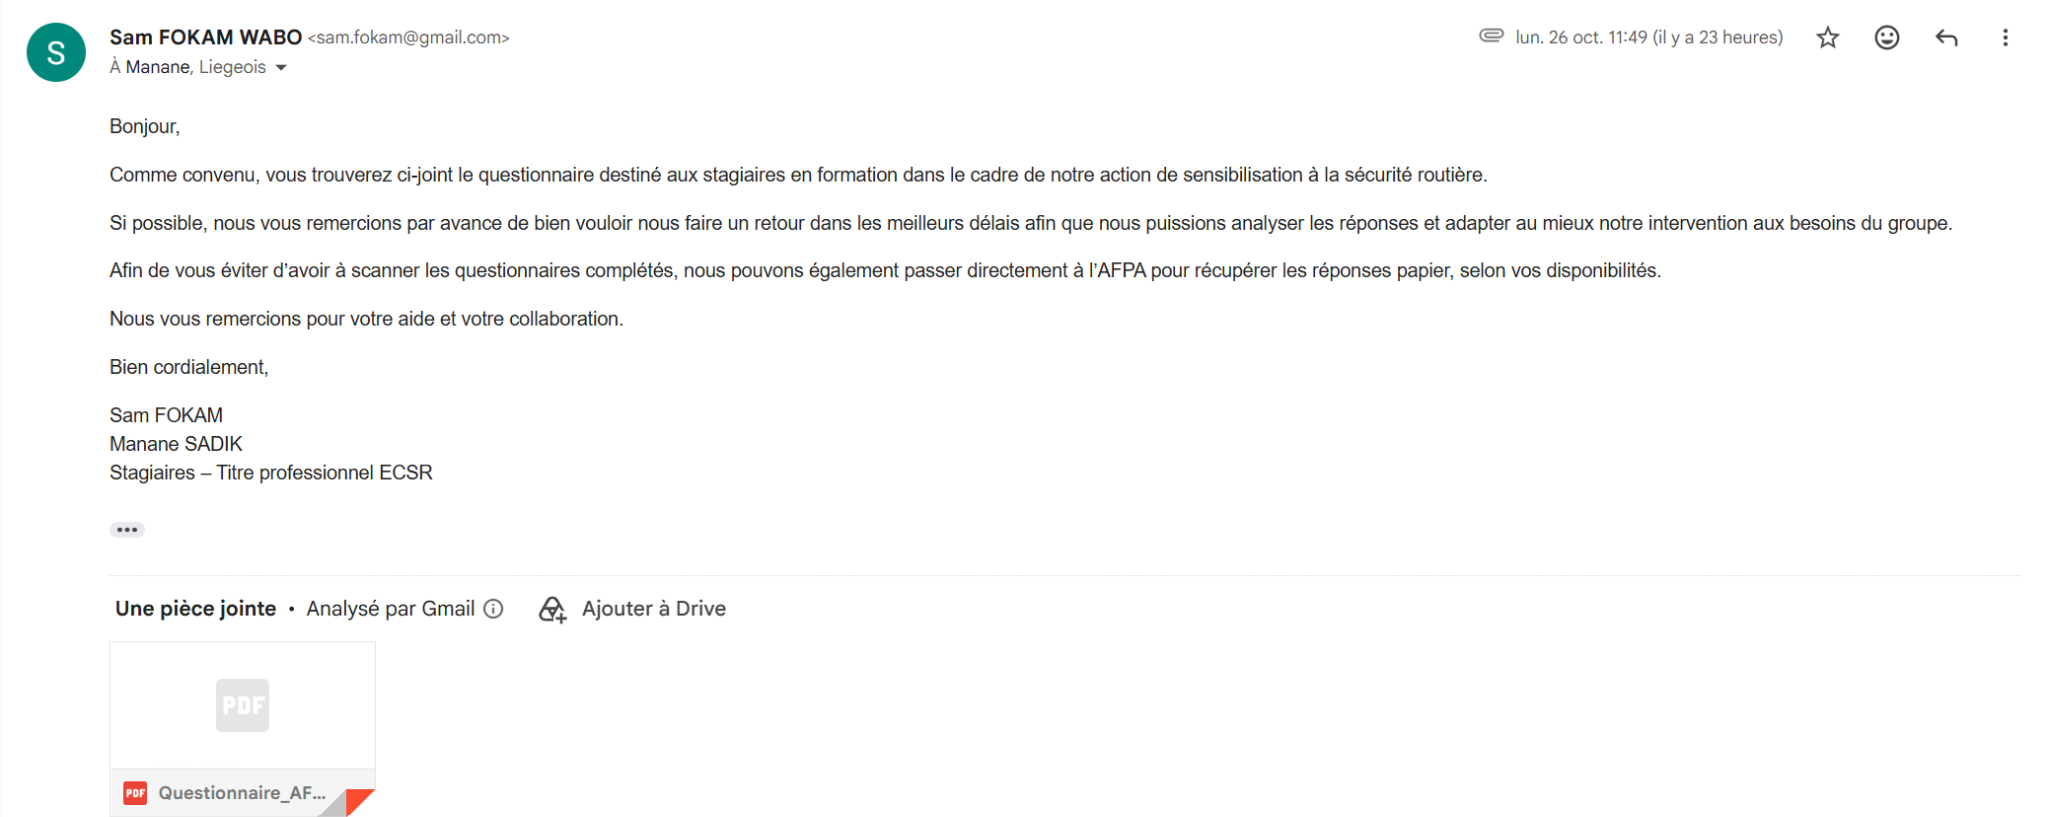
\includegraphics[width=0.97\linewidth,height=0.77\textheight,keepaspectratio]{images/annexes/echanges/a13_20261026_questionnaire_stagiaires.png}
\end{center}
\end{landscape}

\clearpage
\begin{landscape}
\thispagestyle{plain}
\noindent{\large\bfseries 26 octobre — Accord de diffusion au groupe}\par\medskip
\begin{center}
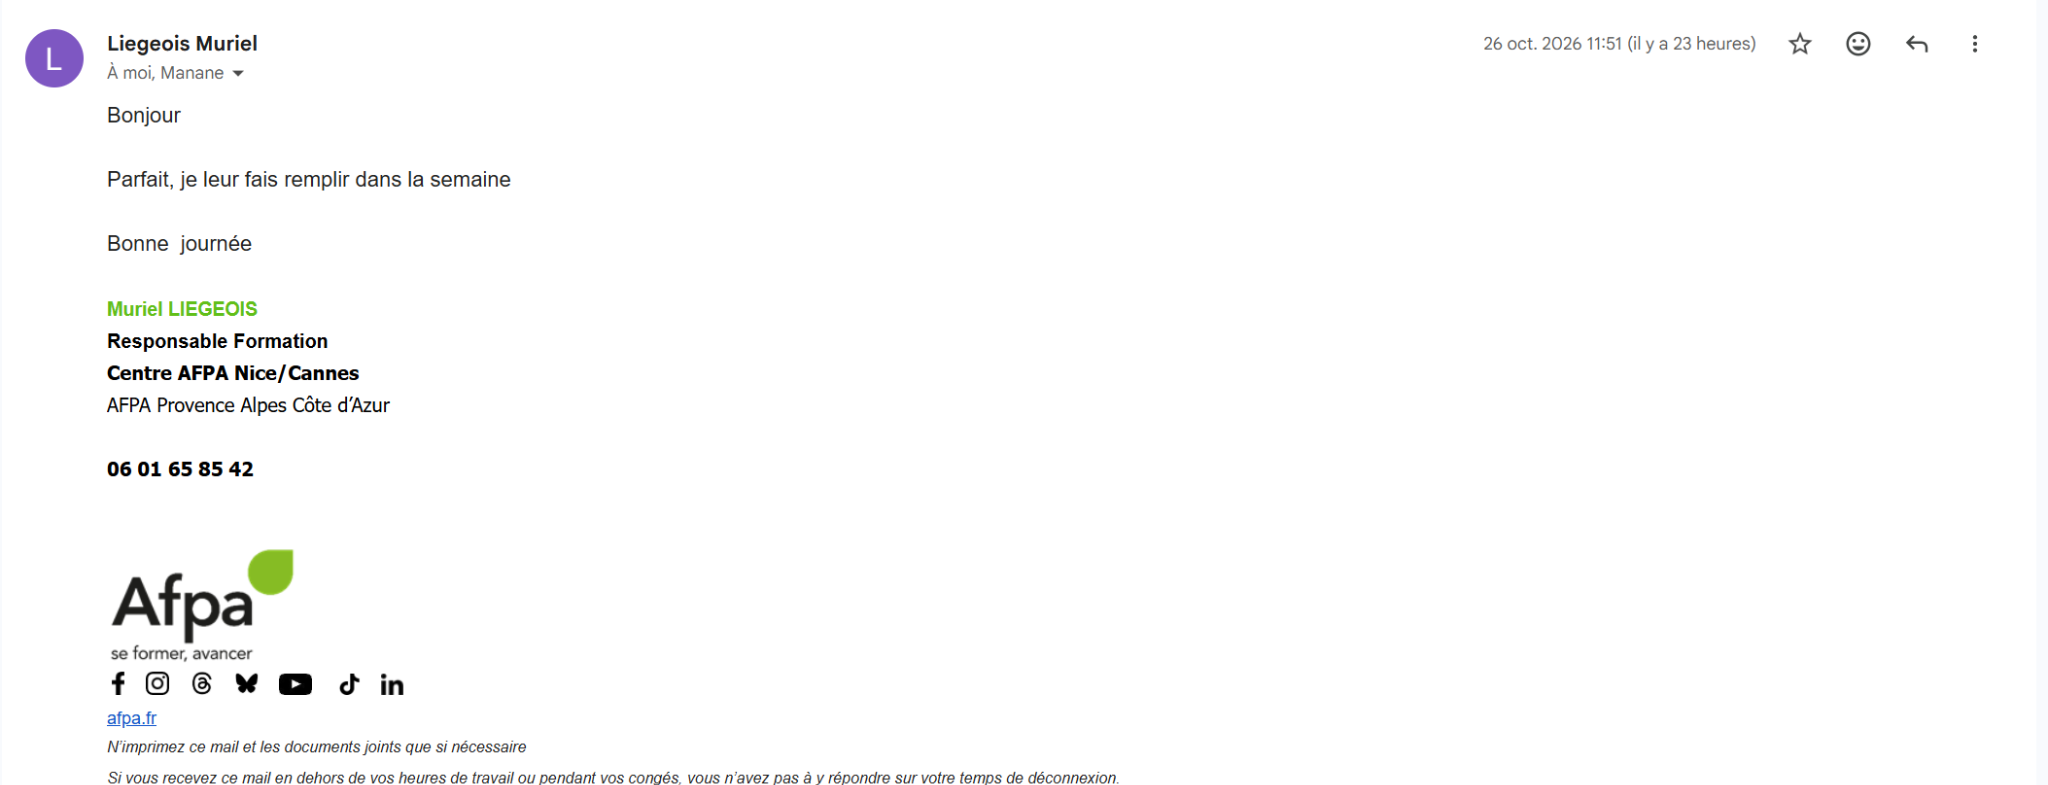
\includegraphics[width=0.97\linewidth,height=0.77\textheight,keepaspectratio]{images/annexes/echanges/a14_20261026_accord_diffusion.png}
\end{center}
\end{landscape}

\clearpage
\begin{landscape}
\thispagestyle{plain}
\noindent{\large\bfseries 29 octobre — Relance pour les réponses}\par\medskip
\begin{center}
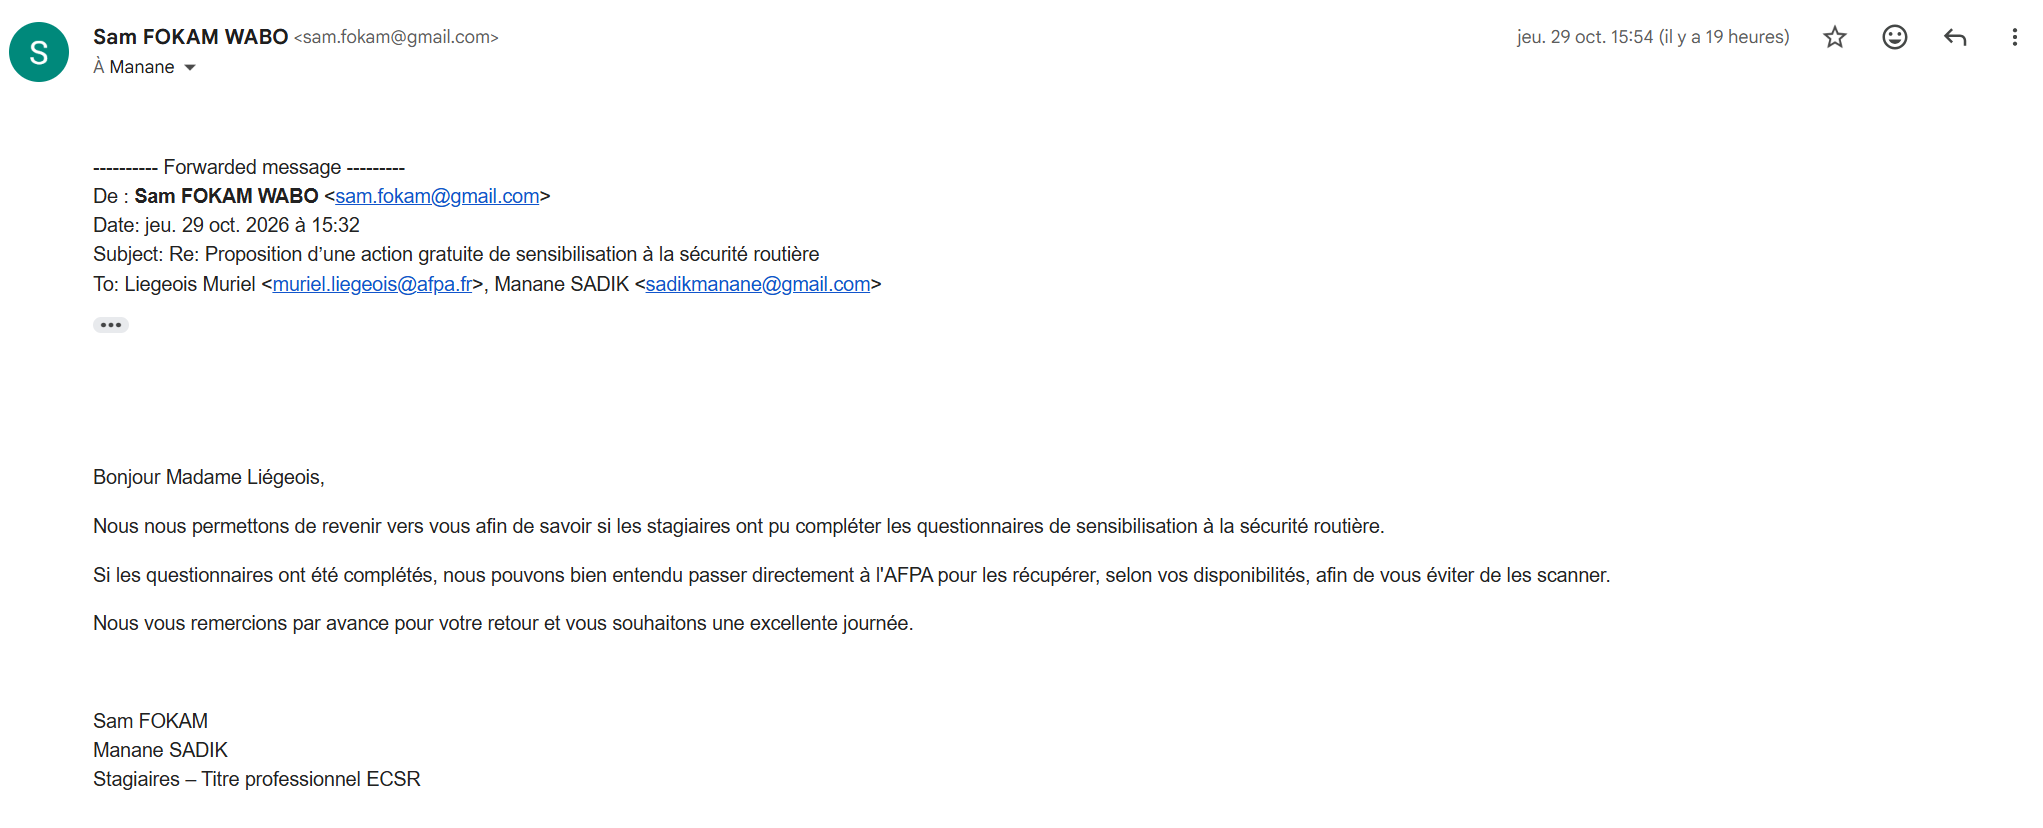
\includegraphics[width=0.97\linewidth,height=0.77\textheight,keepaspectratio]{images/annexes/echanges/a15_20261029_relance.png}
\end{center}
\end{landscape}

\clearpage
\begin{landscape}
\thispagestyle{plain}
\noindent{\large\bfseries 29 octobre — Réponse du commanditaire sur la numérisation}\par\medskip
\begin{center}
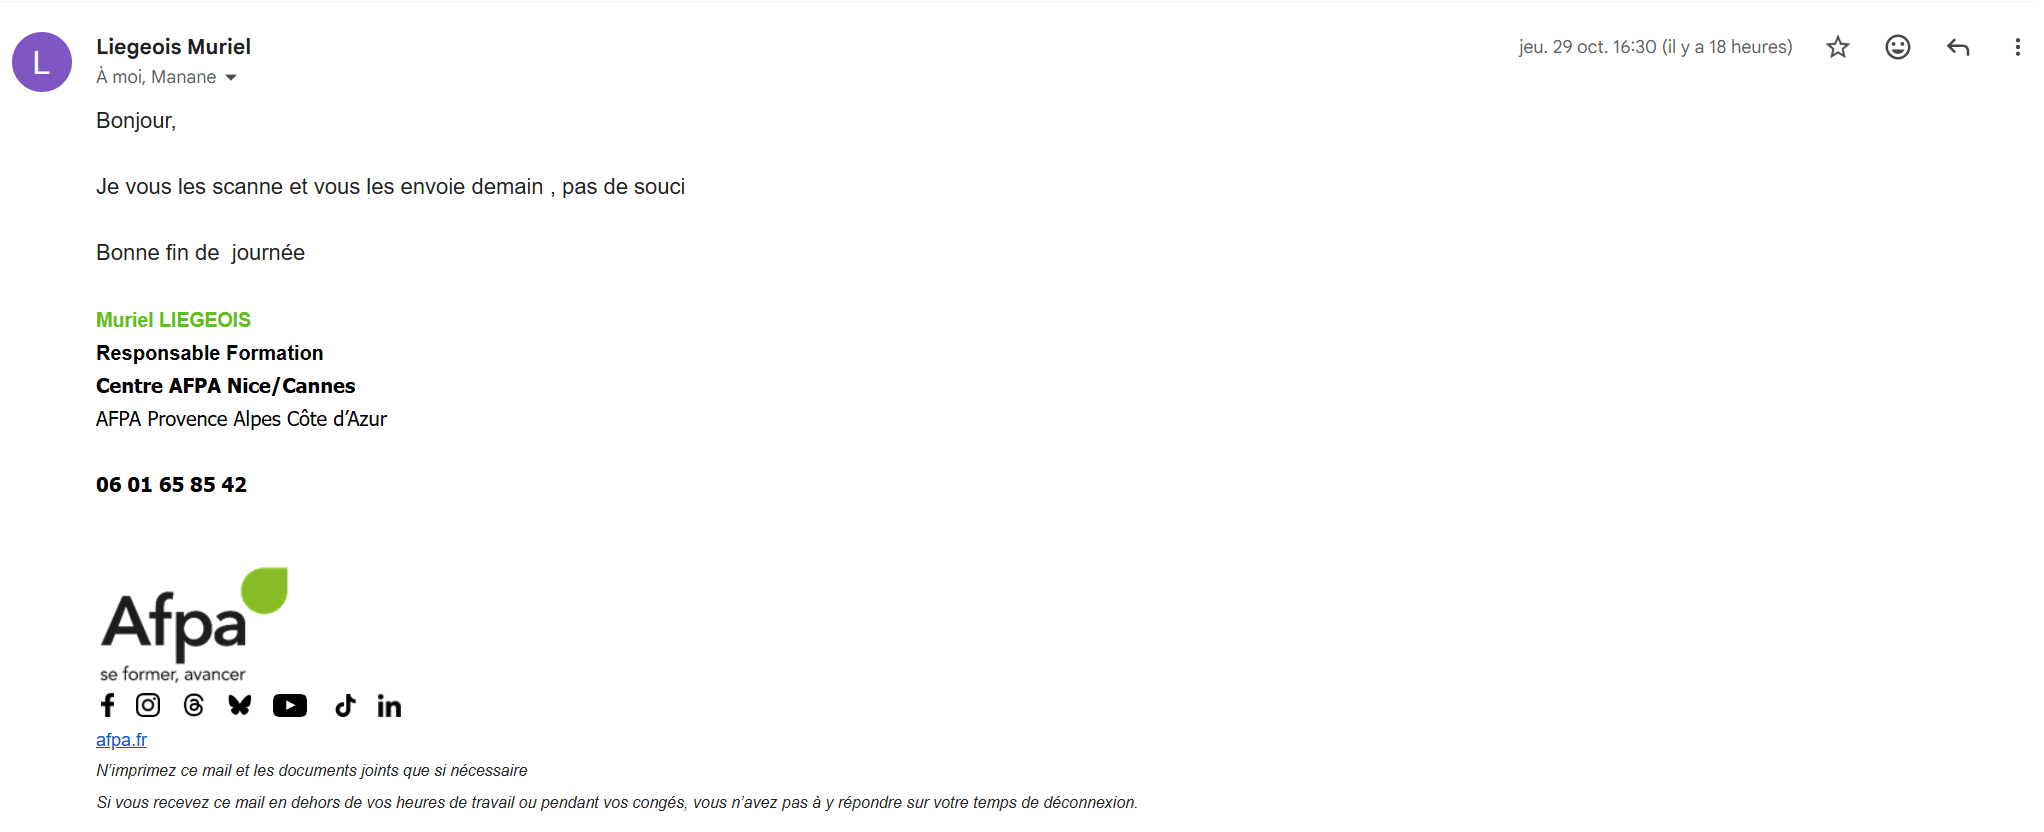
\includegraphics[width=0.97\linewidth,height=0.77\textheight,keepaspectratio]{images/annexes/echanges/a16_20261029_confirmation_retour.png}
\end{center}
\end{landscape}

\section{Recherche de matériel auprès de la Préfecture (A7)}
Correspondance avec le Bureau de la sécurité routière et démarche initiale de conventionnement.

\clearpage
\begin{landscape}
\thispagestyle{plain}
\noindent{\large\bfseries 11 octobre — Sollicitation du Bureau de la sécurité routière}\par\medskip
\begin{center}
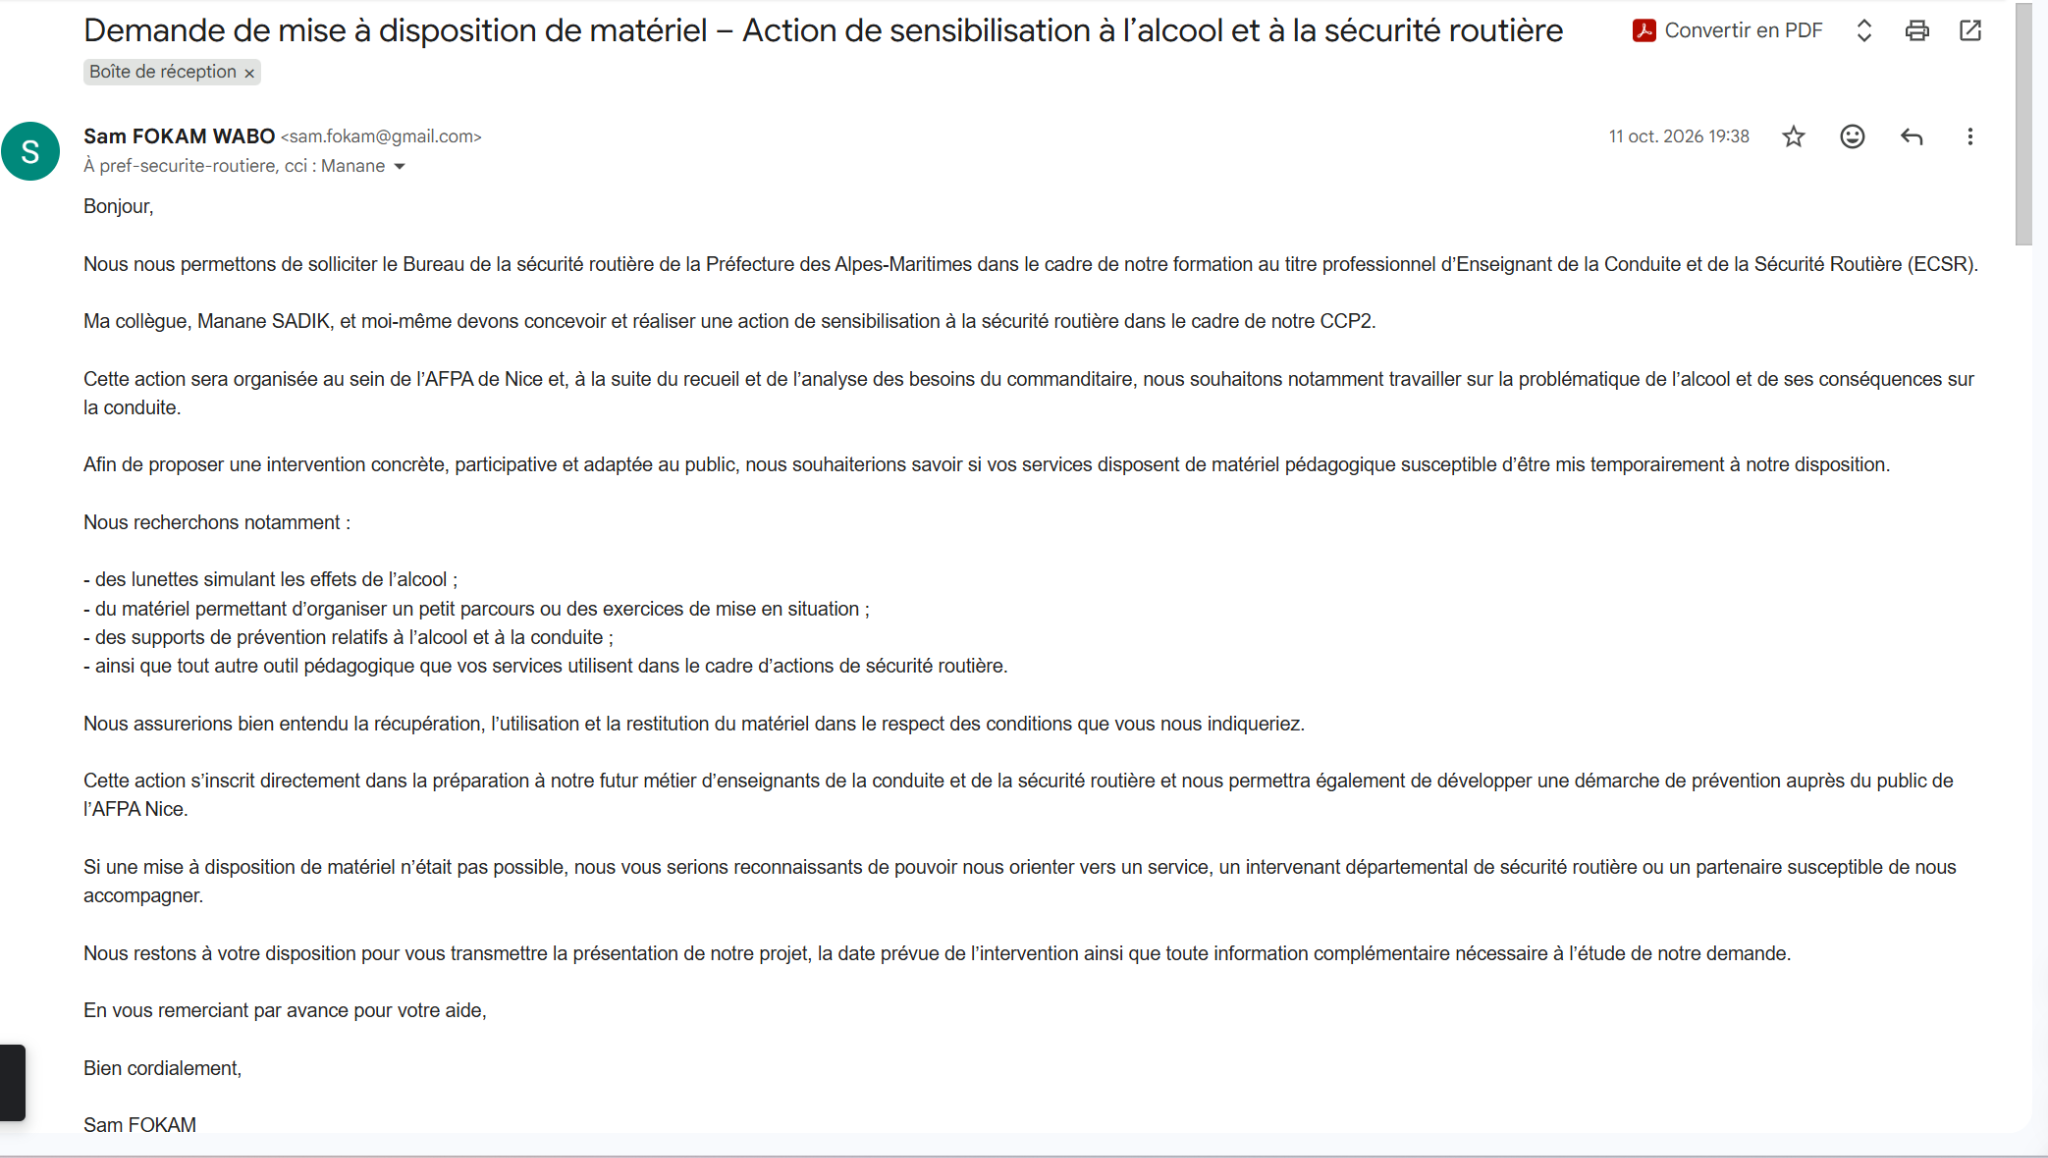
\includegraphics[width=0.97\linewidth,height=0.77\textheight,keepaspectratio]{images/annexes/echanges/p01_20261011_demande_materiel.png}
\end{center}
\end{landscape}

\clearpage
\begin{landscape}
\thispagestyle{plain}
\noindent{\large\bfseries 12 octobre — Proposition de matériel par la Préfecture}\par\medskip
\begin{center}
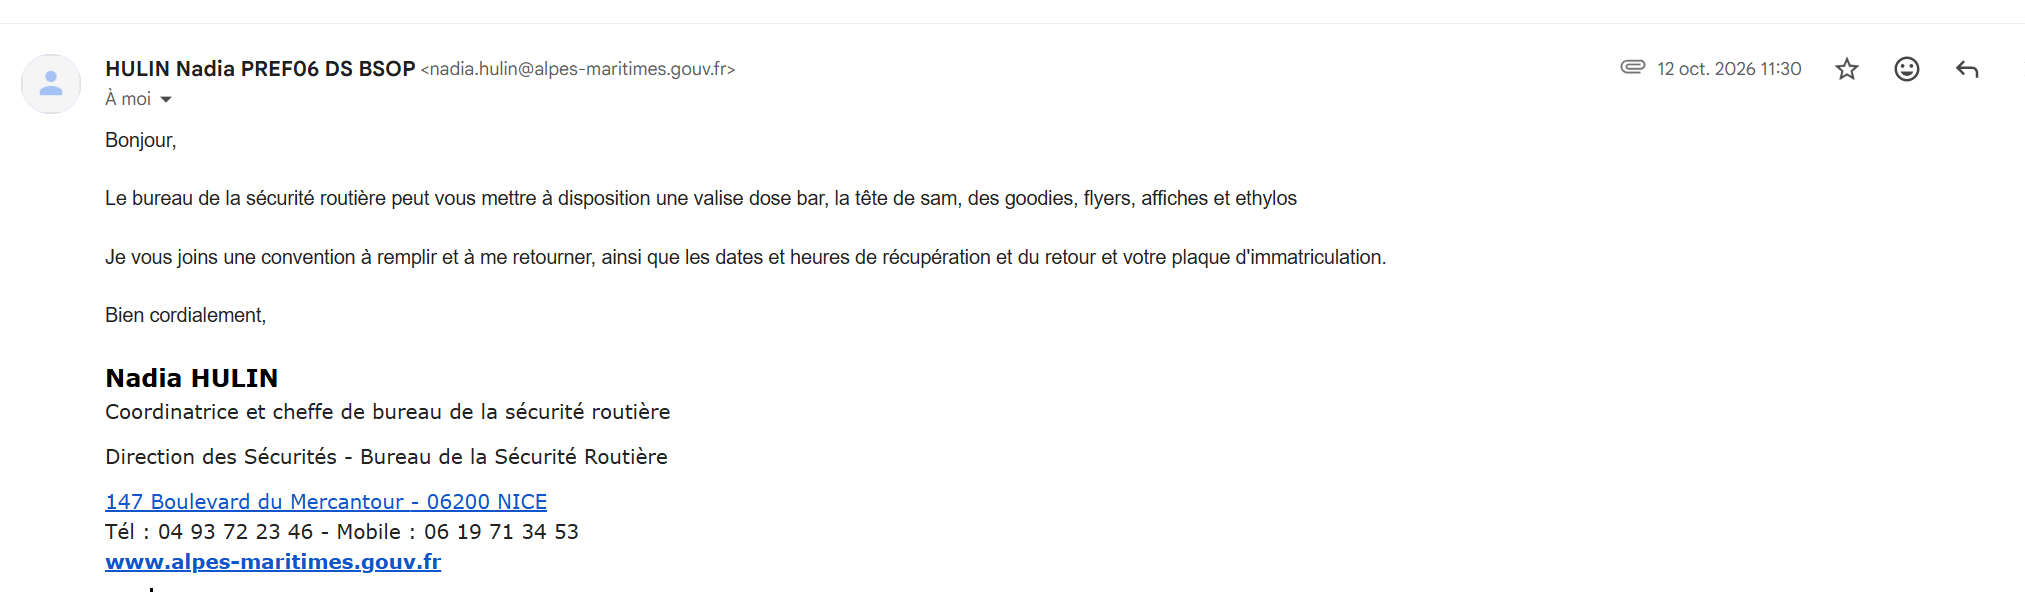
\includegraphics[width=0.97\linewidth,height=0.77\textheight,keepaspectratio]{images/annexes/echanges/p02_20261012_reponse_prefecture.png}
\end{center}
\end{landscape}

\clearpage
\begin{landscape}
\thispagestyle{plain}
\noindent{\large\bfseries 30 octobre — Envoi de la convention signée}\par\medskip
\begin{center}
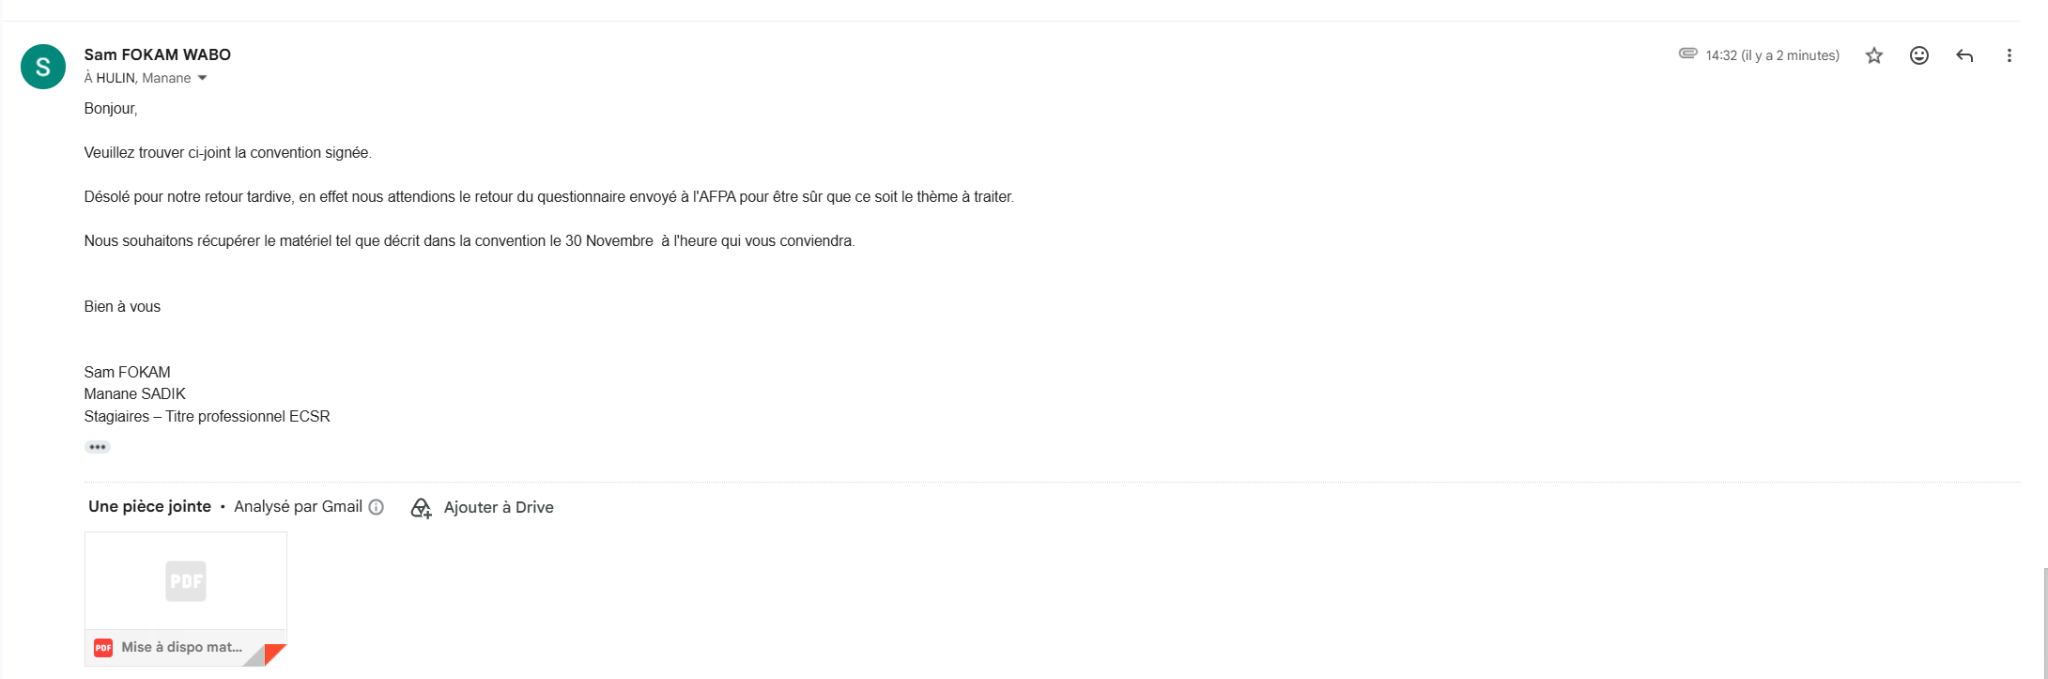
\includegraphics[width=0.97\linewidth,height=0.77\textheight,keepaspectratio]{images/annexes/echanges/p03_20261030_convention_signee.png}
\end{center}
\end{landscape}

\section{Convention et accès logistique au CADAM (A8)}
Échanges relatifs à la signature, aux dates de retrait et de restitution et à la demande d’accès au site. Les opérations effectives restent à confirmer.

\clearpage
\begin{landscape}
\thispagestyle{plain}
\noindent{\large\bfseries 10 novembre — Convention contresignée et changement de retrait}\par\medskip
\begin{center}
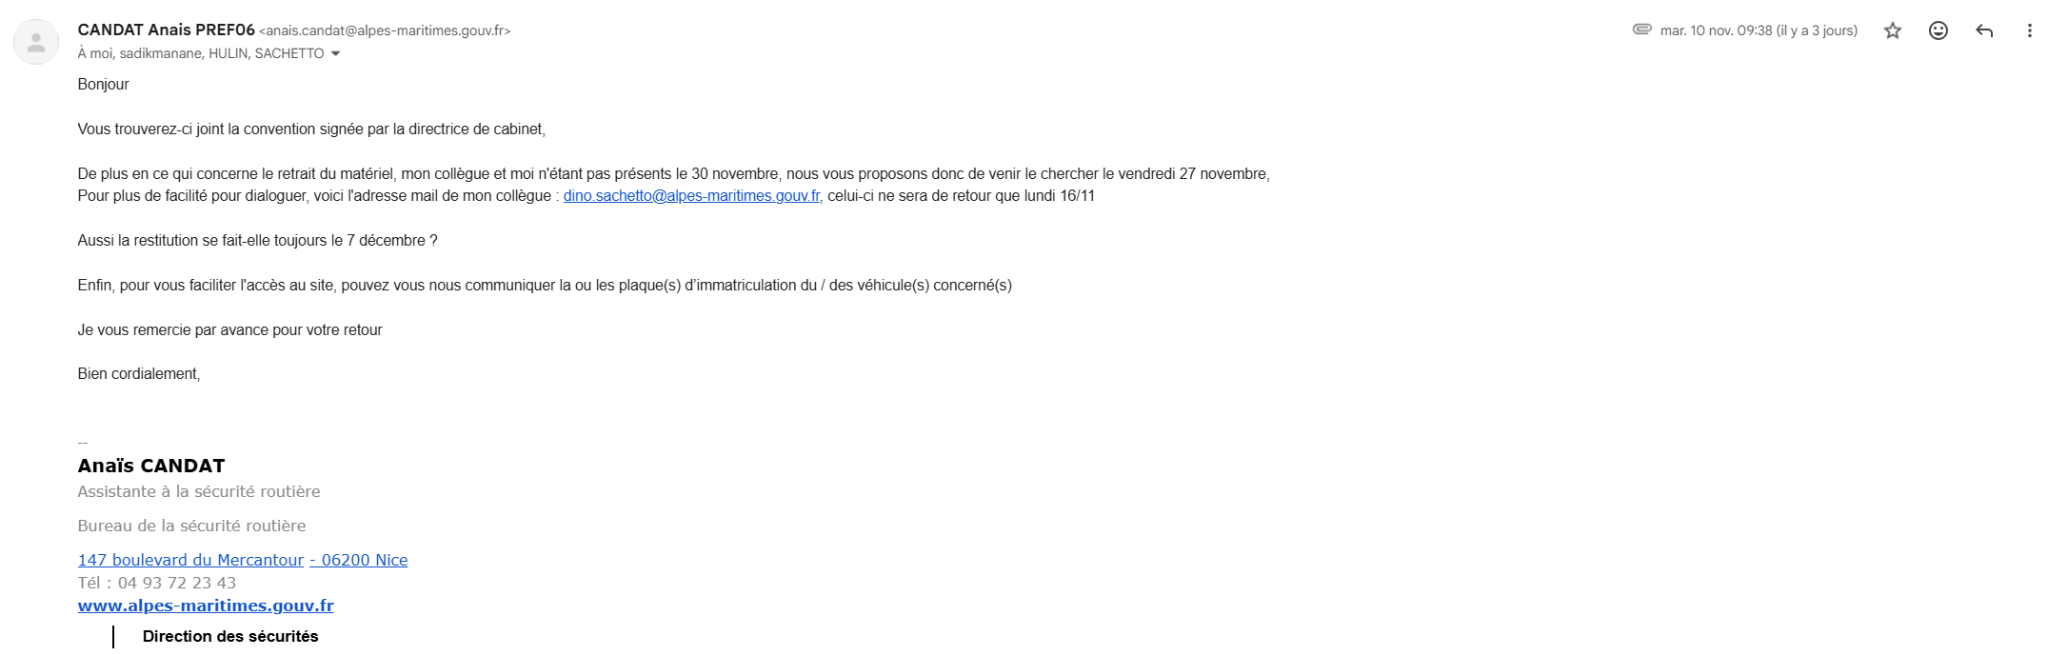
\includegraphics[width=0.97\linewidth,height=0.77\textheight,keepaspectratio]{images/annexes/echanges/p04_20261110_convention_prefecture.png}
\end{center}
\end{landscape}

\clearpage
\begin{landscape}
\thispagestyle{plain}
\noindent{\large\bfseries 10 novembre — Accord sur les nouvelles dates}\par\medskip
\begin{center}
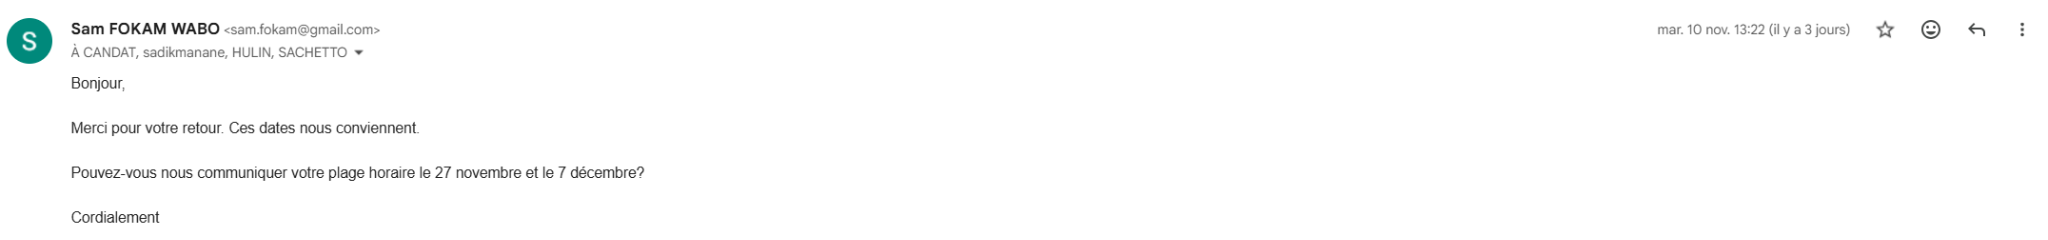
\includegraphics[width=0.97\linewidth,height=0.77\textheight,keepaspectratio]{images/annexes/echanges/p05_20261110_confirmation_dates.png}
\end{center}
\end{landscape}

\clearpage
\begin{landscape}
\thispagestyle{plain}
\noindent{\large\bfseries 12 novembre — Précisions des horaires d’accueil}\par\medskip
\begin{center}
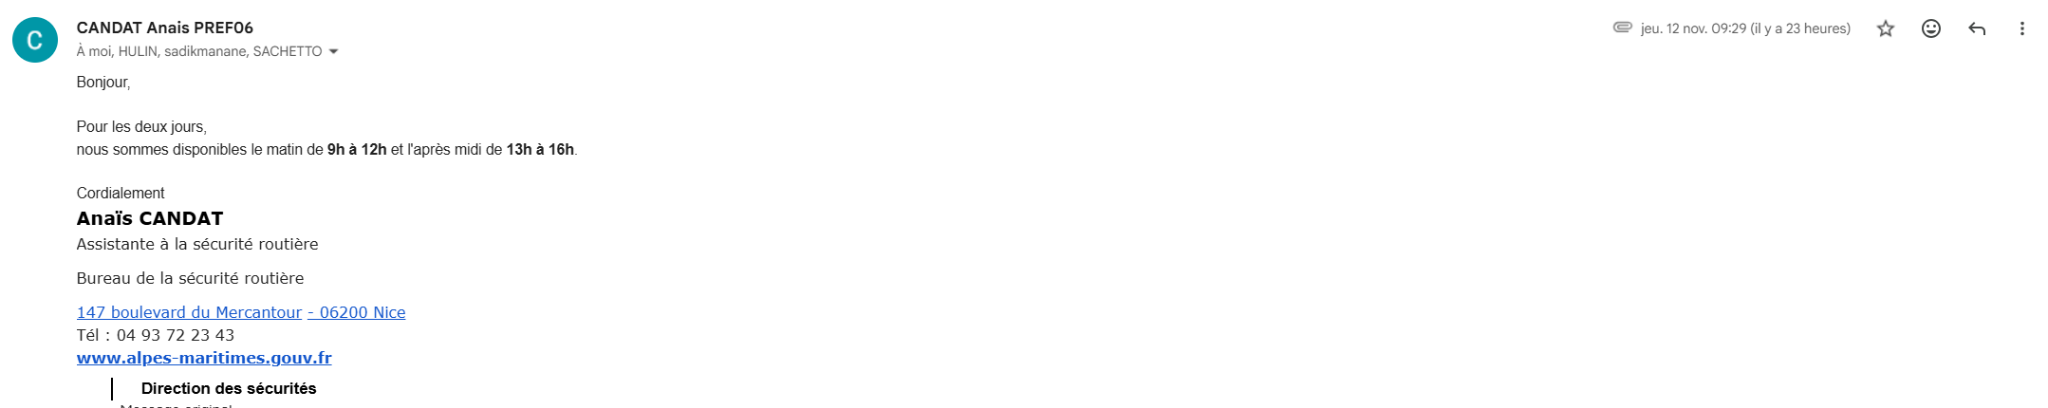
\includegraphics[width=0.97\linewidth,height=0.77\textheight,keepaspectratio]{images/annexes/echanges/p06_20261112_plages_horaires.png}
\end{center}
\end{landscape}

\clearpage
\begin{landscape}
\thispagestyle{plain}
\noindent{\large\bfseries 12 novembre — Confirmation de la matinée et du véhicule}\par\medskip
\begin{center}
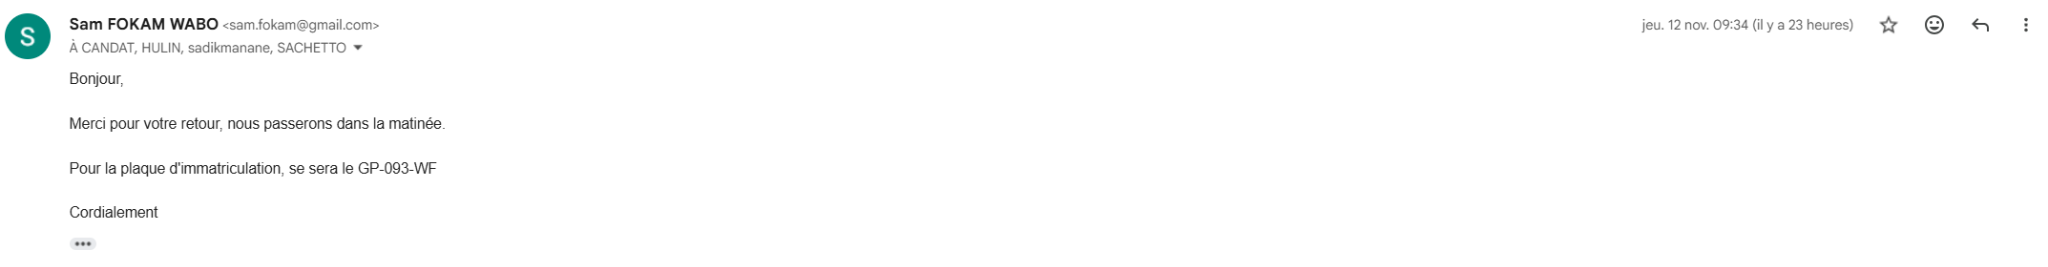
\includegraphics[width=0.97\linewidth,height=0.77\textheight,keepaspectratio]{images/annexes/echanges/p07_20261112_immatriculation.png}
\end{center}
\end{landscape}

\clearpage
\begin{landscape}
\thispagestyle{plain}
\noindent{\large\bfseries 12 novembre — Demande d’accès annoncée}\par\medskip
\begin{center}
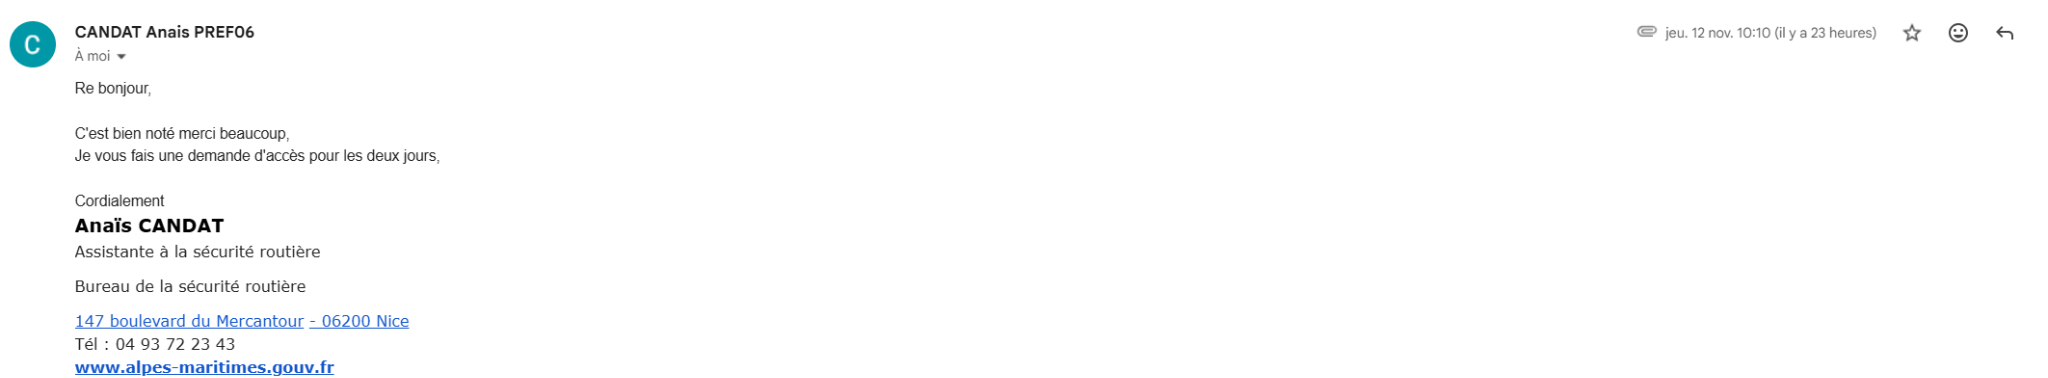
\includegraphics[width=0.97\linewidth,height=0.77\textheight,keepaspectratio]{images/annexes/echanges/p08_20261112_demande_acces.png}
\end{center}
\end{landscape}

\clearpage
\begin{landscape}
\thispagestyle{plain}
\noindent{\large\bfseries 12 novembre — Formalisation de la demande d’accès au CADAM}\par\medskip
\begin{center}
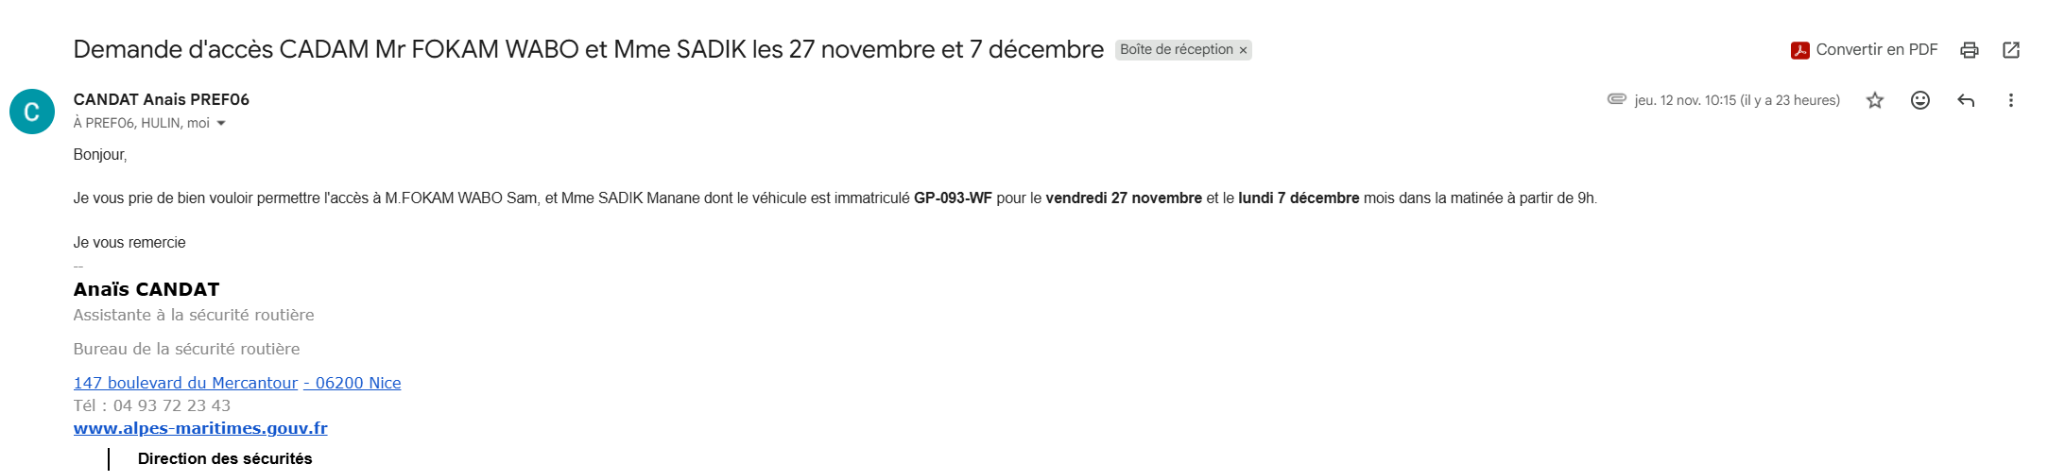
\includegraphics[width=0.97\linewidth,height=0.77\textheight,keepaspectratio]{images/annexes/echanges/p09_20261112_acces_cadam.png}
\end{center}
\end{landscape}

\section{Repères de correspondance avec le CCP2}
\begin{description}[leftmargin=2.9cm,style=nextline]
\item[Compétence 8] Analyse de la demande : prospection, clarification, questionnaire commanditaire et diagnostic du public (chapitres II à IV).
\item[Compétence 9] Construction et préparation : objectifs, moyens, partenaires, scénario et tableau synoptique (chapitre IV).
\item[Compétence 10] Animation de la séance : déroulement effectif et évaluation des acquis (chapitre V, après intervention).
\item[Compétence 11] Analyse de pratique et évolution professionnelle : retour réflexif, remédiations et veille (chapitres VI et VII).
\end{description}

\section{Pièces à intégrer avant remise}
\texteguide{Joindre, dans la version finale uniquement, les pièces autorisées et anonymisées. Privilégier les extraits pertinents : le fichier de réponses individuelles brutes reste un document de travail et n'a pas à être annexé avec ses horodatages.}
